\documentclass[11pt]{article}

\usepackage[T1]{fontenc}
\usepackage[utf8]{inputenc}
\usepackage{lmodern}
\usepackage{microtype}
\usepackage[a4paper,margin=2.35cm]{geometry}
\usepackage{amsmath,amssymb}
\usepackage{booktabs}
\usepackage{array}
\usepackage{tabularx}
\usepackage{multirow}
\usepackage{subcaption}
\usepackage{float}
\usepackage{enumitem}
\usepackage{graphicx}
\usepackage{xcolor}
\usepackage[numbers,sort&compress]{natbib}
\usepackage[hidelinks]{hyperref}

\setlist[itemize]{leftmargin=1.45em,itemsep=0.25em,topsep=0.35em}
\setlength{\bibsep}{2pt}
\setlength{\parskip}{0.15em}
\setlength{\parindent}{1.5em}

\newcommand{\system}{\textsc{Materials Research Agent}}
\newcommand{\hermes}{\textsc{Hermes}}
\newcommand{\matspec}{\textsc{MatSpec}}
\newcommand{\matevidence}{\textsc{MatEvidence}}
\newcommand{\mattransform}{\textsc{MatTransform}}
\newcommand{\matdag}{\textsc{MatDAG}}
\newcommand{\matevolve}{\textsc{MatEvolve}}
\newcommand{\fullsupport}{\ensuremath{\checkmark}}
\newcommand{\partialsupport}{\ensuremath{\circ}}
\newcommand{\notsupport}{--}

\title{\Large\textbf{Materials Research Agent:}\\[0.15em]
\Large\textbf{A Hermes-Based Agentic System for Evidence-Grounded}\\
\Large\textbf{Materials Hypothesis Generation and Structure Exploration}}

\author{
  \textbf{Yiming Hua}\\[0.2em]
  Wuhan University\\
  \href{mailto:cnhym@foxmail.com}{\texttt{cnhym@foxmail.com}}
}

\date{}

\begin{document}

\maketitle

\begin{abstract}
Materials research requires sustained coordination across scientific literature, materials databases, crystal structures, chemical transformations, and computational models. An effective research agent must preserve the constraints of an open-ended scientific question, align heterogeneous evidence around candidate materials, realize hypotheses as explicit structures, dispatch domain models, and carry the resulting artifacts into subsequent rounds of exploration. Existing scientific agents and materials-design systems provide important parts of this process, but commonly treat hypothesis generation, structure manipulation, and computational validation as separate activities. We present \system, a persistent materials-research system built on the \hermes\ agent runtime. \hermes\ provides natural-language interaction, the agent--tool loop, Profile and Skill execution, and controlled research evolution; a Materials MCP Gateway connects this runtime to a structure-centred scientific service. The service is organized around five modules: \matspec\ compiles research goals into scientific constraint graphs; \matevidence\ aligns literature and federated database evidence; \mattransform\ realizes soft-chemistry hypotheses through executable structure operations and condition plans; \matdag\ assembles model-grounded scientific workflows; and \matevolve\ maintains candidate lineages and research artifacts across iterations. We study the system on three end-to-end problems: constraint-guided exploration of two-dimensional transition-metal flat-band structures, multi-route exploration of van der Waals ferromagnetic topological materials, and the open problem of fractional-valence transition metals on a Lieb lattice with a flat band near the Fermi level. Across these studies, the system produces evidence-linked candidate portfolios, parent--child crystal-structure lineages, and prioritized computational and experimental validation trajectories. Together, \hermes\ and the materials-specific scientific layer provide a unified environment in which materials hypotheses can be generated, structurally instantiated, computationally characterized, and progressively refined.
\end{abstract}

\section{Introduction}
\label{sec:introduction}

Materials discovery is a long-horizon coordination problem. A research question expressed in physical or chemical terms must be translated into searchable constraints; relevant mechanisms must be recovered from the literature; candidate identities must be reconciled across databases; proposed modifications must be instantiated as crystal structures; and each structure must be connected to calculations and experiments that can resolve the central hypothesis. Modern infrastructures have made individual parts of this process increasingly powerful. Open materials databases support large-scale retrieval and comparison of computed structures and properties \cite{jain2013materials,haastrup2018c2db}. Graph neural networks and generative models have expanded the accessible crystal-structure space \cite{merchant2023gnome,zeni2025mattergen}, while geometry-constrained generation has begun to target motifs of direct interest to quantum materials, including Lieb lattices \cite{okabe2026scigen}. Autonomous laboratories further connect computational targets, literature-derived synthesis knowledge, active learning, and robotic experimentation \cite{szymanski2023alab}. These advances create a rich collection of scientific resources; using them coherently requires a system that preserves the scientific object and its evidence across the full exploration process.

Large language models provide a natural interface for such coordination. Tool-augmented systems including ChemCrow and Coscientist have shown that an agent can combine language reasoning with chemical software, information retrieval, and laboratory operations \cite{bran2024chemcrow,boiko2023coscientist}. Multi-agent scientific systems have extended this idea to hypothesis generation, proposal refinement, and scientist-in-the-loop discovery \cite{gottweis2026coscientist}. Full-lifecycle systems such as AutoSci frame automated research as a persistent process involving execution, memory, and system evolution rather than a sequence of isolated prompts \cite{qian2026autosci}. In materials science, physics-aware multi-agent systems have connected retrieval, simulation, and multimodal analysis for alloy design \cite{ghafarollahi2024atomagents}. Collectively, these efforts establish the value of agents as organizers of scientific work.

The materials domain, however, places a distinctive requirement on this emerging research paradigm: a hypothesis must remain attached to a physical structure. A statement such as \emph{replace a heavy element to strengthen spin--orbit coupling}, \emph{intercalate an electron donor between magnetic layers}, or \emph{tune the filling of a transition-metal Lieb lattice} is scientifically useful when it is connected to an identified parent structure, a well-defined operation, a resulting child structure or condition plan, and a validation target. The same candidate may be supported by a database record, motivated by a mechanism reported in the literature, transformed through several soft-chemistry operations, and evaluated by multiple models with different input domains. A text-only research trace obscures these dependencies. A structure-centred trace makes them explicit and allows the next model, calculation, or expert decision to operate on the same scientific object.

Existing systems address complementary portions of this problem. General agent runtimes provide interaction, tools, memory, and reusable skills. Scientific lifecycle systems organize literature, experimentation, writing, and review. Chemistry agents connect language models to specialist tools and laboratories. Materials models generate structures or predict particular properties. Table~\ref{tab:system-comparison} compares representative systems at this boundary. The comparison is deliberately feature-level: it asks whether a capability is an explicit, reusable part of the documented system, rather than whether it could be approximated in a single language-model interaction.

\begin{table}[t]
    \centering
    \caption{\textbf{Feature-level comparison of representative scientific-agent and materials-design systems.}}
    \label{tab:system-comparison}
    \small
    \setlength{\tabcolsep}{3.2pt}
    \renewcommand{\arraystretch}{1.16}
    \resizebox{\linewidth}{!}{%
    \begin{tabular}{lccccc}
        \toprule
        \textbf{System} &
        \shortstack{\textbf{Research}\\\textbf{harness}} &
        \shortstack{\textbf{Candidate-linked}\\\textbf{evidence}} &
        \shortstack{\textbf{Executable}\\\textbf{structure lineage}} &
        \shortstack{\textbf{Capability-aware}\\\textbf{model DAG}} &
        \shortstack{\textbf{Persistent}\\\textbf{scientific state}} \\
        \midrule
        ChemCrow \cite{bran2024chemcrow}                  & \partialsupport & \partialsupport & \notsupport    & \notsupport    & \notsupport \\
        Coscientist \cite{boiko2023coscientist}           & \partialsupport & \partialsupport & \notsupport    & \notsupport    & \notsupport \\
        A-Lab \cite{szymanski2023alab}                    & \fullsupport    & \partialsupport & \partialsupport & \partialsupport & \partialsupport \\
        AtomAgents \cite{ghafarollahi2024atomagents}      & \partialsupport & \partialsupport & \partialsupport & \partialsupport & \notsupport \\
        MatterGen / SCIGEN \cite{zeni2025mattergen,okabe2026scigen}
                                                            & \notsupport    & \notsupport    & \partialsupport & \notsupport    & \notsupport \\
        AutoSci \cite{qian2026autosci}                    & \fullsupport    & \partialsupport & \notsupport    & \partialsupport & \fullsupport \\
        \textbf{Materials Research Agent (ours; Hermes-based)}
                                                            & \fullsupport    & \fullsupport    & \fullsupport    & \fullsupport    & \fullsupport \\
        \bottomrule
    \end{tabular}%
    }
    \vspace{0.25em}

    \begin{minipage}{0.98\linewidth}
        \footnotesize
        Symbols denote full support (\fullsupport), partial or task-/campaign-local support (\partialsupport), and capabilities that are not a primary focus (\notsupport). A research harness requires controlled multi-stage tool execution rather than tool access alone. Candidate-linked evidence requires literature and database observations to be joined to stable material identities with retained provenance. Executable structure lineage requires typed operations or condition plans with explicit parent--child relationships; producing isolated structures is counted as partial support. A capability-aware model DAG binds candidate-specific observables to registered models or calculations and their dependencies. Persistent scientific state denotes reusable evidence, structures, tasks, and decisions beyond a single dialogue or execution trace. The symbols describe system scope, not comparative scientific performance.
    \end{minipage}
\end{table}

The comparison exposes a division of labour. Chemistry agents provide broad tool use and experimental planning; A-Lab closes a synthesis loop for predefined inorganic targets; AtomAgents couples multi-agent reasoning to atomistic simulation; MatterGen and SCIGEN produce explicit crystals under property or motif constraints; and AutoSci supplies a general research harness with structured persistent memory. None of these systems makes candidate-linked evidence, executable soft-chemistry structure lineage, capability-aware model workflows, and persistent scientific state parts of the same materials-research abstraction. The resulting opportunity is to join these capabilities around a durable candidate representation that binds scientific constraints, evidence sources, structure lineage, model tasks, and subsequent validation. This is the systems-level problem studied in this work.

From this perspective, a materials-research agent should satisfy six requirements.

\begin{enumerate}[leftmargin=1.75em,label=\textbf{R\arabic*.},itemsep=0.45em]
    \setcounter{enumi}{-1}
    \item \textbf{Persistent agent runtime.}
    The system should support natural-language interaction, long-running tool use, reusable task policies, and research continuity across turns.

    \item \textbf{Compilable scientific goals.}
    An open-ended request should become a structured set of compositional, structural, electronic, magnetic, realizability, and evidence constraints, together with permitted operations and validation targets.

    \item \textbf{Federated evidence.}
    Literature mechanisms, database properties, source structures, and model-derived observations should be aligned around stable candidate identities while retaining their provenance.

    \item \textbf{Structure-backed hypotheses.}
    Scientific proposals should be realized through explicit parent--child structures or condition plans. Relevant operations include site substitution, vacancy formation, intercalation, strain, layer sliding, carrier doping, electrostatic gating, magnetic proximity, and van der Waals heterostructure construction.

    \item \textbf{Capability-aware scientific execution.}
    Candidate-specific questions should be translated into dependency-aware tasks for structure models, Hamiltonian models, band analysis, and first-principles calculations.

    \item \textbf{Evolvable research state.}
    Evidence, structures, computations, and expert decisions should remain reusable across iterations, enabling the system to expand promising structure families and prioritize subsequent calculations or experiments.
\end{enumerate}

To meet these requirements, we introduce \system, a materials-research system built on \hermes\ \cite{nousresearch2026hermes}. \hermes\ serves as the outer agent runtime: it receives a natural-language scientific goal, loads a materials-specific Profile and Skill, invokes reviewed tools, and returns structured results to the researcher. We connect this runtime to a Materials MCP Gateway that exposes coarse-grained research operations while keeping the scientific state in a dedicated materials service. This separation gives the system a clear division of labour. \hermes\ supplies the general interaction and agent substrate; our materials layer supplies evidence-aware reasoning, candidate identities, executable crystal-structure transformations, model task graphs, and scientific artifact memory.

The materials layer contains five cooperating modules. \matspec\ translates a research goal into a constraint graph and search plan. \matevidence\ combines scholarly retrieval with federated materials databases and attaches each observation to a candidate and source. \mattransform\ compiles chemically meaningful hypotheses into five executable structure operations and four condition-level plans, preserving the lineage from every parent structure to its descendants. \matdag\ maps the resulting candidates to model-grounded workflows spanning database electronic structures, machine-learning interatomic models, learned Hamiltonians, band analysis, and first-principles calculations. \matevolve\ maintains the candidate portfolio and scientific artifact graph across iterations. At the runtime level, a separate controlled-evolution Profile can use \hermes-native memory, Skills, and delegation to accumulate reusable workflow experience; at the scientific level, the materials service remains the record of candidate structures, evidence, calculations, and validation state.

Figure~\ref{fig:overview} summarizes the resulting three-layer architecture and research lifecycle. A user-defined materials question enters through \hermes, reaches the scientific modules through MCP, and returns as a portfolio of traceable evidence, structures, tasks, and follow-up decisions. The same architecture supports research questions with markedly different degrees of openness: constrained screening of two-dimensional flat-band candidates; six complementary routes toward van der Waals ferromagnetic topological materials; and a three-route exploration of fractional-valence transition-metal Lieb lattices.

\begin{figure}[t]
    \centering
    \IfFileExists{figures/system-overview-image2-v1.png}{
        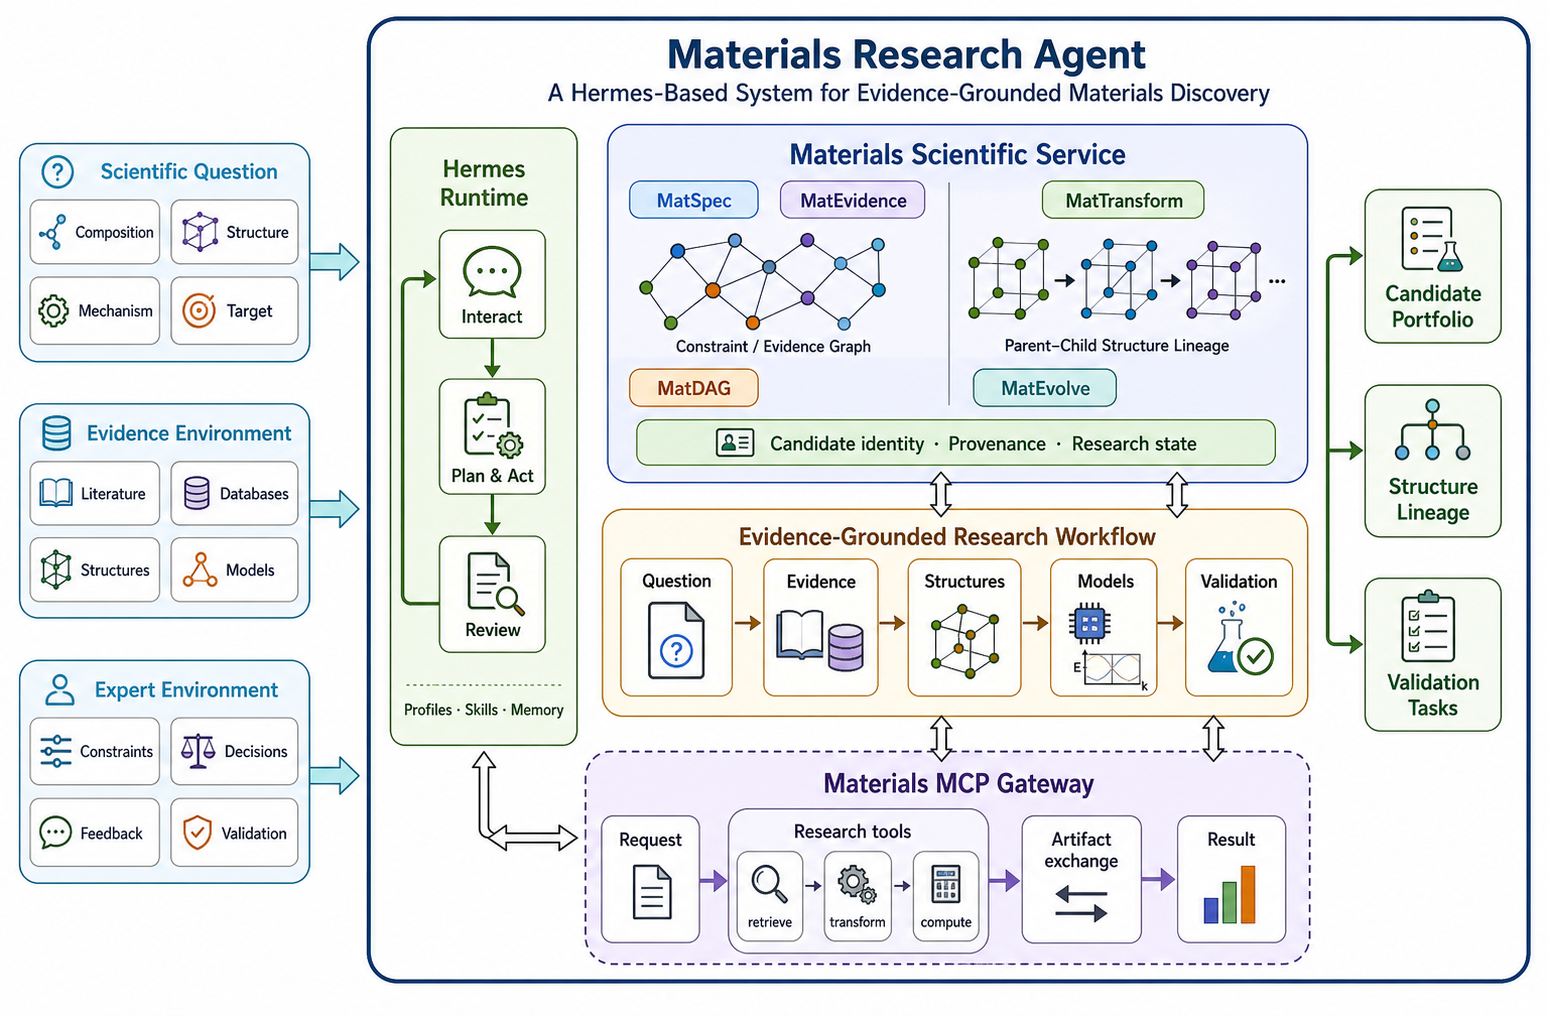
\includegraphics[width=\linewidth]{figures/system-overview-image2-v1.png}
    }{
        \fbox{
            \begin{minipage}{0.92\linewidth}
                \centering
                \vspace{0.5em}
                \hermes\ \textbf{Agent Runtime}\\[-0.1em]
                Natural-language interaction $\cdot$ Agent--tool loop $\cdot$
                Profiles/Skills $\cdot$ controlled evolution\\[0.45em]
                $\Downarrow$\\[-0.15em]
                \textbf{Materials MCP Gateway}\\[-0.1em]
                Research submission $\cdot$ run state $\cdot$
                scientific artifact exchange\\[0.45em]
                $\Downarrow$\\[-0.15em]
                \textbf{Materials Scientific Service}\\[-0.1em]
                \matspec\ $\rightarrow$ \matevidence\ $\rightarrow$
                \mattransform\ $\rightarrow$ \matdag\ $\rightarrow$ \matevolve\\[0.45em]
                $\Downarrow$\\[-0.15em]
                Evidence-linked candidates $\cdot$ parent--child structures
                $\cdot$ model tasks $\cdot$ validation trajectories
                \vspace{0.5em}
            \end{minipage}
        }
    }
    \caption{\textbf{Overview of Materials Research Agent.}
    \hermes\ provides the interaction and agent runtime, a Materials MCP Gateway connects the runtime to domain tools, and five materials-science modules transform an open-ended research goal into evidence-linked candidate structures and validation tasks. Scientific artifacts are returned to the runtime for expert review and subsequent research iterations.}
    \label{fig:overview}
\end{figure}

Our main contributions are:

\begin{itemize}
    \item \textbf{A Hermes-based materials-research architecture.}
    We extend the \hermes\ agent runtime with source-controlled materials Profiles and Skills, a Materials MCP interface, and a structure-centred scientific service, establishing an explicit boundary between reusable agent capabilities and domain-specific scientific operations.

    \item \textbf{A unified formulation of evidence, structures, and validation.}
    We formulate materials hypothesis generation as the joint evolution of a scientific constraint graph, a federated evidence graph, a candidate structure lineage, and a capability-aware validation graph.

    \item \textbf{An end-to-end scientific implementation.}
    We implement literature and database federation, nine soft-chemistry structure or condition operations, candidate-level scientific task DAGs, model execution interfaces, and persistent research artifacts that connect each hypothesis to its parent structure and next validation step.

    \item \textbf{Three materials case studies and a layered evaluation design.}
    We apply the same system to two-dimensional flat-band exploration, van der Waals ferromagnetic topological materials, and fractional-valence Lieb lattices. The evaluation separates the contribution of the base language model, the \hermes\ runtime, materials evidence tools, structure operations, and the complete \hermes-based materials system.
\end{itemize}

The remainder of this paper first describes the \hermes-based system architecture and its interface to the materials service, then presents the five scientific modules, followed by the three case studies and their cross-case evaluation.

\section{System Overview}
\label{sec:system}

\subsection{Design principle: the candidate is the unit of research}

\system treats a materials campaign as the evolution of a set of scientific objects rather than the generation of a sequence of answers.  The central object is a \emph{candidate record}.  It binds a stable material identity to five kinds of state: the constraints against which the candidate is judged, the evidence supporting those judgements, the parent or generated crystal structure, the computations scheduled for that structure, and the decisions that determine its subsequent trajectory.  A candidate may begin as a database structure, a literature mechanism, or a model-proposed composition.  In each case, the same record is enriched rather than replaced as the campaign progresses.

This representation is useful because materials questions are usually underdetermined at the moment they are posed.  A database may establish that a structure is two-dimensional but contain no evidence about the orbital character of a band; a paper may motivate a mechanism without providing a machine-readable structure; and a generated child may be geometrically valid before its electronic state is known.  The system therefore permits incomplete candidate records while requiring every populated field to retain its source.  Missing observations remain explicit targets for subsequent work.

\begin{figure}[t]
    \centering
    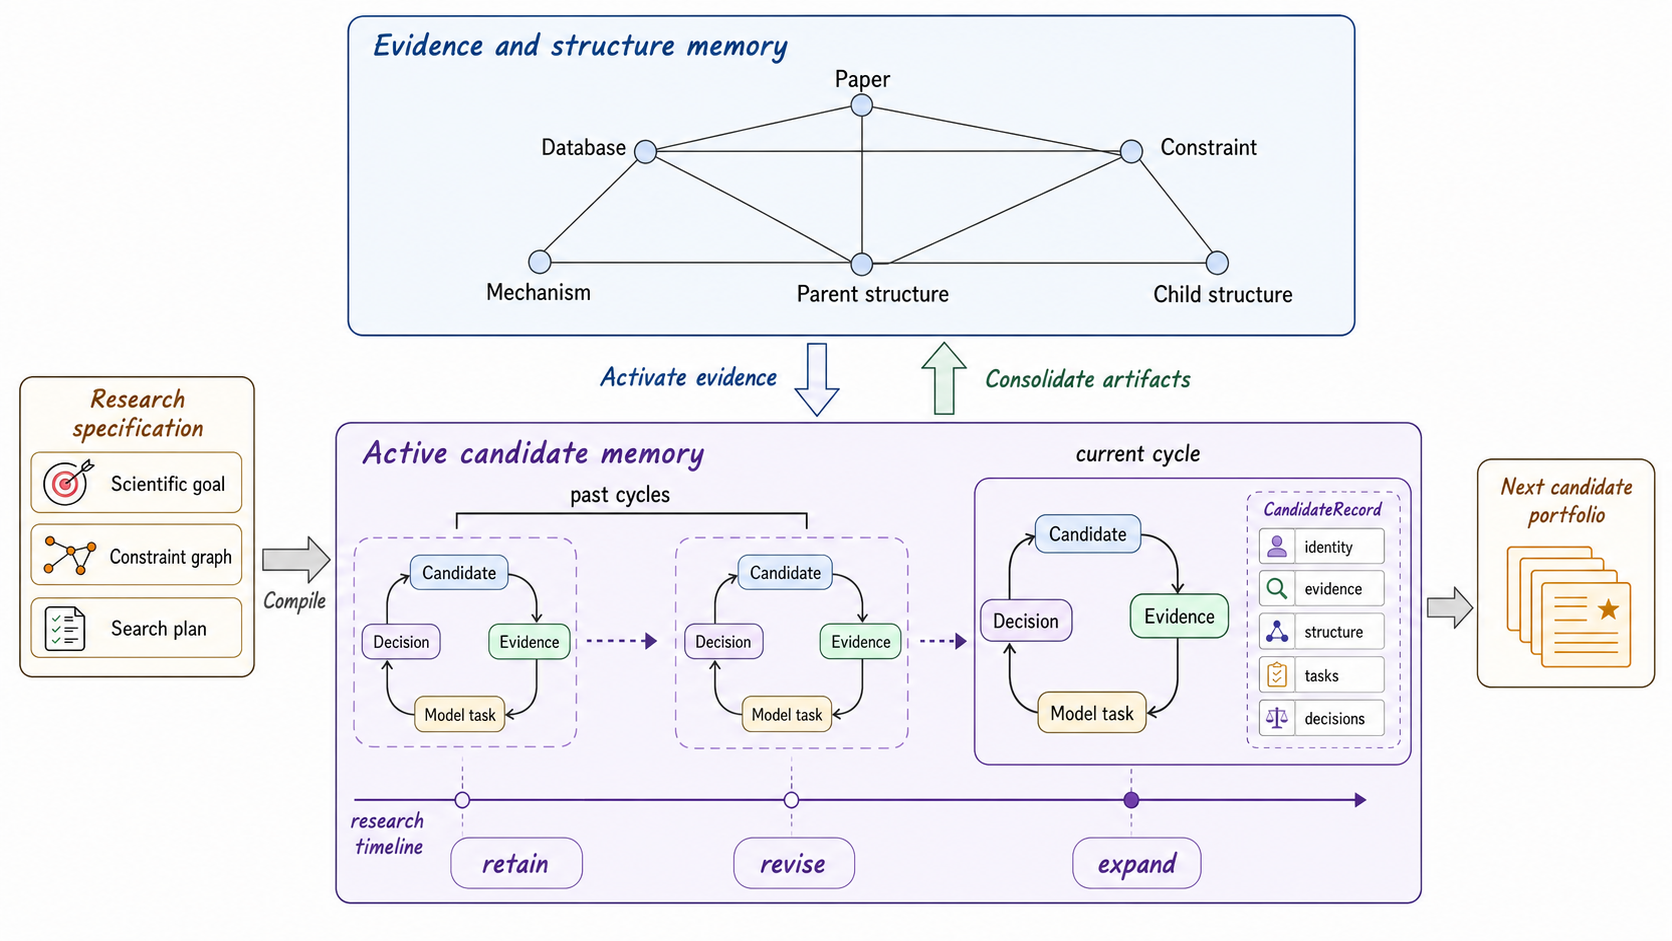
\includegraphics[width=\linewidth]{figures/candidate-artifact-graph-image2-v2.png}
    \caption{\textbf{Candidate-centred scientific memory.}
    Candidate-independent evidence and structures occupy a durable scientific memory, whereas active candidate cycles bind evidence, model tasks, and decisions to a \texttt{CandidateRecord}.  Activation supplies relevant prior artifacts to the current cycle; consolidation writes validated structures and observations back into the shared graph.}
    \label{fig:artifact-graph}
\end{figure}

Figure~\ref{fig:artifact-graph} shows the resulting artifact graph.  An \texttt{EvidenceRecord} stores an observation, its source, retrieval or calculation metadata, and the constraint it can address.  A \texttt{StructureRecord} stores a canonical structure artifact and any transformation that relates it to a parent.  A \texttt{ModelTask} binds an observable to a registered capability and to its input and dependency artifacts.  A \texttt{DecisionRecord} records whether the system retains, revises, or expands a candidate.  These records are individually addressable and are joined through stable candidate identifiers, rather than being embedded only in a final natural-language report.

\subsection{Hermes as the outer research runtime}

\hermes is the outer execution environment of the platform.  A source-controlled \hermes Profile defines the tools visible to the agent, approval policy, time and concurrency limits, and the Skills that specify how a materials campaign is conducted.  The production Profile exposes only bounded materials tools: starting a research run, reading run state, applying an advertised action, reading a verified terminal result, and launching the generic materials-research pipeline.  General terminal, browser, file, and code-execution tools are disabled in this Profile.  This makes the scientific service---rather than an unstructured agent workspace---the authority for candidate state.

The runtime contributes four capabilities.  First, it translates a natural-language goal into a tool-mediated research interaction without requiring the researcher to call individual scientific programs.  Second, it supports long-running runs through explicit state inspection and resumable actions.  Third, it loads distinct materials Profiles for production research, research-only exploration, and controlled evolution.  Fourth, its native memory, Skills, and bounded delegation can be enabled in the evolution Profile to accumulate reusable workflow knowledge while the underlying scientific records remain read-only from that Profile.

This separation is important.  \hermes memory describes how to conduct research; the materials service records what is known about a particular candidate.  The former can improve reusable workflow policy.  The latter preserves structures, evidence, computations, and decisions with scientific provenance.  The two memories interact through reviewed summaries and stable artifact references, but they do not replace one another.

\subsection{The Materials MCP Gateway}

The Materials Model Context Protocol (MCP) Gateway is a narrow interface between the agent runtime and the scientific service.  Its tools use strict input and output schemas and return bounded projections of internal state.  Mutating actions are separated from read-only state and result retrieval.  A run cannot return a terminal result until the authoritative report and its referenced artifacts have been verified by the service.  Requests are idempotently keyed by submission or run identifiers so that an interrupted \hermes interaction can recover an existing campaign instead of silently creating a second one.

The gateway deliberately exposes coarse-grained scientific operations.  For example, the generic materials-research tool initiates the complete evidence and hypothesis workflow; it does not expose a free-form sequence of database queries as independent agent actions.  The underlying service fans out to configured sources, compiles evidence matrices, plans transformations, and constructs model tasks.  This design retains the convenience of natural-language research while keeping identity resolution, scientific verdicts, and structure mutation in deterministic or typed components.

\begin{table}[t]
    \centering
    \caption{\textbf{Division of responsibility between the agent runtime and scientific service.}}
    \label{tab:responsibility}
    \small
    \setlength{\tabcolsep}{5pt}
    \renewcommand{\arraystretch}{1.15}
    \begin{tabularx}{\linewidth}{>{\raggedright\arraybackslash}p{0.18\linewidth}XX}
        \toprule
        \textbf{Layer} & \textbf{Primary responsibility} & \textbf{Persistent output} \\
        \midrule
        \hermes runtime & Dialogue, Profile/Skill policy, agent--tool loop, bounded continuation and workflow evolution & Session state, reusable workflow memory, reviewed Skill updates \\
        Materials MCP Gateway & Schema validation, run admission, action boundary, status and artifact projection & Run identity, action receipts, verified result handles \\
        Materials service & Constraint compilation, evidence federation, structure operations, scientific DAGs and candidate decisions & Candidate, evidence, structure, task and decision records \\
        Scientific backends & Database retrieval, structural checks, learned models, band analysis and first-principles calculations & Source artifacts, model outputs, numerical observations and execution receipts \\
        \bottomrule
    \end{tabularx}
\end{table}

\subsection{End-to-end lifecycle}

A campaign proceeds through five stages.  (1) \matspec compiles the question into typed constraints, permitted modifications, and target observables.  (2) \matevidence retrieves literature and database records, resolves candidate identities, and builds an evidence matrix.  (3) \mattransform converts selected hypotheses into typed structure-operation or condition plans and, where possible, explicit child structures.  (4) \matdag binds candidates to capability-checked model tasks and executes the resulting dependency graph.  (5) \matevolve combines the new artifacts with the current portfolio and produces the next candidate set and validation trajectory.

The lifecycle is not a rigid linear pipeline.  A candidate can return from \matdag to \matevidence when a calculation creates an observation that resolves a previously unknown constraint.  It can return to \mattransform when a result motivates a revised substitution, strain state, or heterostructure.  It can also branch into several descendants while retaining a common parent.  The invariant is that each transition produces a typed artifact and that no observation is detached from the candidate and structure to which it applies.

\subsection{Implementation}

The scientific service is implemented in Python using strict versioned data models.  Structures are stored as content-addressed artifacts, and canonical JSON payloads are hashed to construct deterministic plan identifiers.  The current system includes federated adapters for C2DB, Materials Cloud MC3D, NOMAD, and Materials Project; structure manipulation through an independent soft-chemistry registry; and scientific executors for database electronic structures, structure and energy models, learned Hamiltonians, band analysis, and remote first-principles calculations.  Append-only run directories retain requests, source responses, normalized records, task plans, execution receipts, plots, and reports.  The experiments in Section~\ref{sec:experiments} use these stored artifacts rather than reconstituted examples.

\section{MatSpec: Compiling Open-Ended Materials Questions}
\label{sec:matspec}

Materials questions often mix hard requirements, mechanistic preferences, permitted interventions, and desired measurements in one sentence.  \matspec separates these roles and compiles the request into a scientific constraint graph
\begin{equation}
    \mathcal{G}_{\mathrm{spec}}=(\mathcal{C},\mathcal{R},\mathcal{O},\mathcal{Y}),
\end{equation}
where $\mathcal{C}$ is a set of typed constraints, $\mathcal{R}$ contains logical or mechanistic relations between constraints, $\mathcal{O}$ specifies allowed structure or condition operations, and $\mathcal{Y}$ lists the observables required to evaluate the goal.  The graph is the contract shared by retrieval, hypothesis generation, transformation, and validation.

\subsection{Constraint types}

Each constraint $c_i\in\mathcal{C}$ contains a type, subject, predicate, threshold or categorical target, evidence requirement, and priority.  We use six broad types: composition, crystal structure, electronic structure, magnetism and topology, chemical realizability, and evidence quality.  A hard constraint determines whether a candidate can satisfy the stated problem; a ranking constraint distinguishes promising candidates within the feasible set; and a context constraint records a mechanism or condition needed to interpret other observations.  The distinction prevents a strong literature mechanism from being mistaken for a measured candidate property, while still allowing it to guide search.

\begin{table}[t]
    \centering
    \caption{\textbf{Examples of MatSpec constraint compilation in the three case studies.}}
    \label{tab:constraints}
    \small
    \setlength{\tabcolsep}{4pt}
    \renewcommand{\arraystretch}{1.13}
    \begin{tabularx}{\linewidth}{>{\raggedright\arraybackslash}p{0.15\linewidth}>{\raggedright\arraybackslash}p{0.23\linewidth}X>{\raggedright\arraybackslash}p{0.18\linewidth}}
        \toprule
        \textbf{Problem} & \textbf{Constraint} & \textbf{Compiled interpretation} & \textbf{Target evidence} \\
        \midrule
        2D flat band & Transition-metal sublattice & A periodic connected graph of transition-metal sites must remain in the explicit structure & Canonical CIF and graph analysis \\
        2D flat band & Flat band near $E_\mathrm{F}$ & Bandwidth and Fermi-level distance are distinct observables; neither is inferred from metadata & Band energies on a declared $k$ path \\
        vdW FM topology & Intrinsic or engineered ferromagnetism & Separate magnetic ground state, ordering scale, and magnetic-anisotropy targets & Magnetic calculations or experiment \\
        vdW FM topology & Non-trivial topology & SOC gap, Fermi-level placement and topological invariant are separate constraints & SOC Hamiltonian/DFT and invariant \\
        Lieb lattice & Fractional transition-metal valence & Formal charge balance must admit a non-integer average $d$-metal valence without asserting site-resolved charge order & Composition, structure and later charge analysis \\
        Lieb lattice & Lieb connectivity & Contributor sites must form the intended line-centred-square graph rather than a visually similar motif & Structure graph and orbital projection \\
        \bottomrule
    \end{tabularx}
\end{table}

Table~\ref{tab:constraints} illustrates a central aspect of compilation: compound phrases are split into independently testable observables.  ``Ferromagnetic topological insulator'', for example, does not become one Boolean property.  It becomes a conjunction of magnetic order, relevant temperature scale, spin--orbit-coupled gap, Fermi-level placement, and a topological diagnostic.  Similarly, ``a flat band at the Fermi level'' separates bandwidth, energy alignment, competing dispersive crossings, and orbital or sublattice character.

\subsection{Relations and conditional paths}

Edges $\mathcal{R}$ encode logical dependence and scientific mechanism.  A hard logical edge can state that a topological invariant is meaningful only for an identified isolated band manifold.  A mechanistic edge can state that increasing spin--orbit coupling is expected to act on a band inversion, but does not by itself establish topology.  Conditional edges define alternative research routes: intrinsic magnetism, magnetic intercalation, proximity coupling, electrostatic control, strain, or heterostructure formation can each be explored while sharing the same terminal observables.

This representation permits open questions to remain open without becoming vague.  The fractional-valence Lieb-lattice problem, for example, is expressed as three coordinated routes: federated structure discovery, literature-and-mechanism transfer, and direct structure generation.  All three populate a common candidate schema and are judged against the same constraint graph, even though their starting evidence differs.

\subsection{Search and validation plans}

The compiled search plan specifies which sources can directly address each constraint and which observations require new computation.  Source selection is based on declared fields rather than convenience.  If a source supplies a structure but no band energies, it can support dimensionality or connectivity but cannot support the flat-band constraint.  The validation plan maps unresolved constraints to observables and assigns a preferred progression from inexpensive evidence to more specific calculation.  For electronic candidates, a typical progression is database band retrieval, learned-Hamiltonian screening, explicit band diagnostics, and selected first-principles confirmation.  For structural interventions, the plan first requires an executable child structure and hard-gate checks before electronic tasks are admitted.

The output of \matspec is therefore not a prose paraphrase.  It is a versioned graph and a set of machine-checkable targets that constrain every downstream module.  The original user goal is retained alongside its compiled representation so that final reports can connect each claim back to the question that motivated it.

\section{MatEvidence: Federated, Candidate-Linked Evidence}
\label{sec:matevidence}

\matevidence converts heterogeneous scientific sources into evidence records attached to stable candidate identities.  It combines a nine-role research workflow with deterministic source normalization and candidate--constraint matrix construction.  The language model proposes searches, interprets mechanisms, and develops hypotheses; source adapters and schema validators determine what evidence was actually retrieved and which candidate it describes.

\subsection{Nine-role research workflow}

The workflow decomposes research into nine roles: requirements analysis, query planning, native scholarly search, evidence resolution, database scouting, mechanism and chemistry analysis, skeptical constraint review, hypothesis reasoning, and synthesis.  The roles communicate through structured records rather than a shared untyped transcript.  Query planning emits source and concept queries.  Native search returns candidate papers or database leads.  Evidence resolution obtains persistent identifiers and source metadata.  Database scouting returns normalized structure records.  Mechanism analysis connects candidate modifications to the target constraints.  The skeptic populates evidence verdicts, and the hypothesis reasoner produces a separate inference matrix.  The synthesist constructs the final candidate portfolio and next-step plan.

\begin{table}[t]
    \centering
    \caption{\textbf{Roles in the generic materials-research workflow.}}
    \label{tab:roles}
    \small
    \setlength{\tabcolsep}{4pt}
    \renewcommand{\arraystretch}{1.12}
    \begin{tabularx}{\linewidth}{>{\raggedright\arraybackslash}p{0.22\linewidth}XX}
        \toprule
        \textbf{Role} & \textbf{Question answered} & \textbf{Structured output} \\
        \midrule
        Requirements & What is the scientific target? & Constraint graph and ambiguity ledger \\
        Query planner & Which concepts and sources should be searched? & Source-specific query plan \\
        Native search & Which papers and records are plausible leads? & Ranked scholarly and database leads \\
        Evidence resolver & Which persistent objects support the lead? & DOI/arXiv/source records and provenance \\
        Database scout & Which explicit structures instantiate candidates? & Federated candidate and structure records \\
        Mechanism/chemistry & Why might a candidate or intervention work? & Mechanism links and proposed operations \\
        Skeptic & What is directly established for each constraint? & Sparse PASS/FAIL judgements with evidence links \\
        Hypothesis reasoner & What remains plausible despite missing evidence? & LIKELY\_PASS/LIKELY\_FAIL and falsifiers \\
        Synthesist & What should be retained and tested next? & Candidate portfolio and validation trajectory \\
        \bottomrule
    \end{tabularx}
\end{table}

The decomposition limits two common failure modes.  First, a search lead cannot become evidence merely because it is semantically relevant: it must be resolved to a stable source object and linked to the correct candidate.  Second, the same model is not asked to propose a hypothesis and then silently certify it.  The skeptic reconstructs direct evidence, while the reasoner states probabilistic scientific expectations and the observations that would falsify them.

\subsection{Federated materials identities}

The current federation includes C2DB, Materials Cloud MC3D, NOMAD, and Materials Project.  Each adapter stores the source namespace, source identifier, retrieval time, native fields, normalization policy, and source artifact.  Structures are canonicalized and content-hashed; composition and structure fingerprints are used to propose cross-source identity links.  The federation retains the original identities even when two records are linked, because database entries can differ in dimensionality, relaxation protocol, magnetic state, or calculation level.

Source fields are not imputed across candidates or databases.  If MC3D contributes a structure but does not expose an energy-above-hull value in the retrieved record, that constraint remains unknown for that source.  If C2DB supplies a PBE band structure, the observation is labelled with its computational origin rather than treated as an experimental fact.  Cross-source links broaden the evidence available to a candidate, but every observation continues to point to the record that produced it.

\subsection{Evidence and inference are separate matrices}

For candidate $m_j$ and constraint $c_i$, the direct evidence matrix contains
\begin{equation}
    E_{ij}\in\{\mathrm{PASS},\mathrm{FAIL},\mathrm{UNKNOWN}\}.
\end{equation}
A PASS or FAIL requires an evidence record whose scope and value can evaluate the compiled predicate.  UNKNOWN is a first-class outcome: it means that the retrieved artifacts do not decide the constraint.  In parallel, the hypothesis reasoner produces
\begin{equation}
    H_{ij}=(v_{ij},p_{ij},a_{ij},f_{ij}),
\end{equation}
where $v_{ij}\in\{\mathrm{LIKELY\_PASS},\mathrm{LIKELY\_FAIL}\}$, $p_{ij}$ is a calibrated qualitative or numeric confidence, $a_{ij}$ lists assumptions, and $f_{ij}$ is a decisive falsification target.  The final report can therefore say both that a route is scientifically motivated and that a particular observable remains to be measured or computed.

This dual representation is especially important in early materials exploration.  A promising candidate is not discarded because a specialized property is absent from a database, and an attractive mechanism is not promoted to established evidence.  Instead, missing high-value entries in $E$ become candidate-specific validation tasks in \matdag.

\subsection{Candidate and evidence graphs}

Every evidence record contains a relation to the candidate: identity, analogue, parent, child, mechanism support, constraint observation, or negative discriminator.  These relations form a graph that can express, for example, that a paper motivates orbital-selective flat bands in an oxyhalide family; a database record supplies the NbOCl$_2$ parent structure; a substitution plan generates a related child; and a learned Hamiltonian supplies a bandwidth for that exact child.  The graph prevents evidence about the family from being silently assigned to the generated structure.

The output of \matevidence is a candidate set, the complete candidate--constraint evidence matrix, an independent inference review, and a set of unresolved high-value observables.  These objects provide the input to structure realization and model routing.

\section{MatTransform: Executable Soft-Chemistry Hypotheses}
\label{sec:mattransform}

A materials hypothesis becomes actionable when its intervention can be applied to an identified structure.  \mattransform provides a typed grammar that converts scientific proposals into deterministic operation plans.  The grammar distinguishes operations that create a child CIF from condition plans that describe an external or interfacial realization.  Both are retained in the candidate lineage.

\subsection{Structure operations and condition plans}

The implemented registry contains five structure operations: equivalent-site substitution, removal of an equivalent-site class, reasoned intercalation into a gap site, homogeneous strain, and reasoned layer sliding.  It also contains four condition or interface plans: carrier doping, electrostatic gating, magnetic proximity, and van der Waals heterostructure construction.  Figure~\ref{fig:softchem} summarizes the grammar.

\begin{figure}[t]
    \centering
    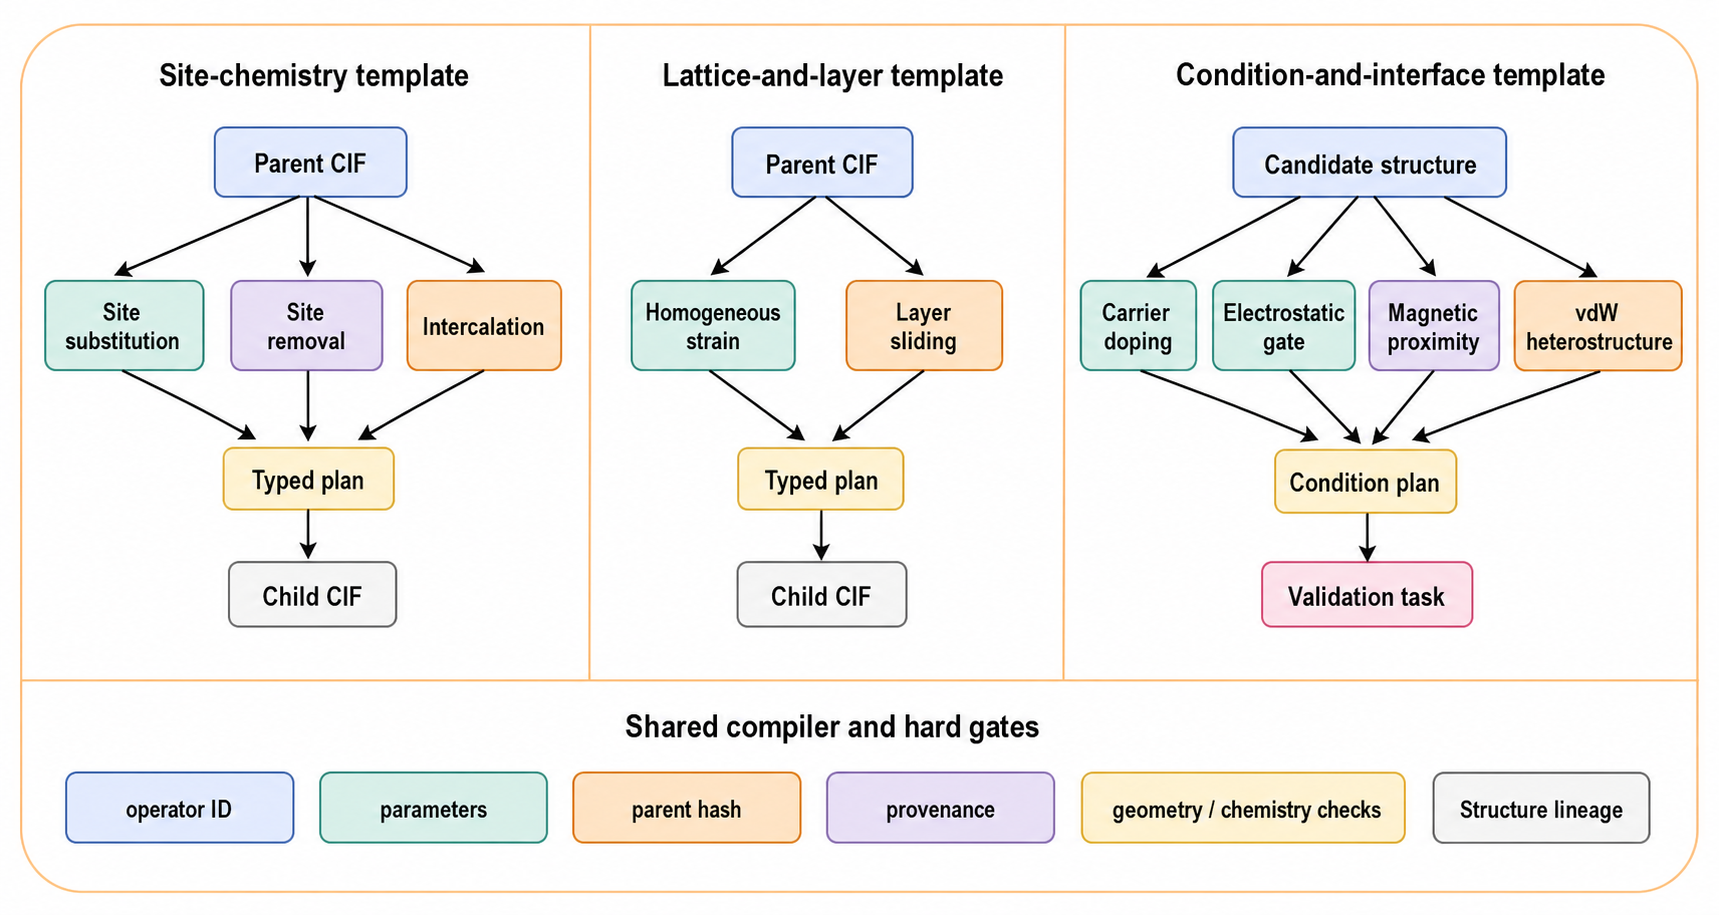
\includegraphics[width=\linewidth]{figures/softchem-grammar-image2-v2.png}
    \caption{\textbf{Stage-specific templates in the executable soft-chemistry grammar.}
    Site chemistry, lattice/layer changes, and condition/interface interventions use separate operator DAGs while sharing a typed compiler, content-hashed parent binding, provenance, and hard-gate layer.  Structure templates terminate in an explicit child CIF; condition templates terminate in a validation task.}
    \label{fig:softchem}
\end{figure}

An operation plan is represented as
\begin{equation}
    o=(\texttt{id},\texttt{version},s_{\mathrm{parent}},\theta,q,\pi),
\end{equation}
where $\theta$ is a typed parameter object, $q$ records the scientific rationale and target constraints, and $\pi$ is the provenance of the proposal.  The plan identifier is derived from canonical serialized content.  Replaying the same operator version and parameters on the same parent therefore recovers the same plan identity; changing the parent, parameters, or version produces a new lineage edge.

Equivalent-site substitution and removal act on a complete symmetry or equivalence class selected in the plan.  This makes site choice explicit and avoids a nominal composition change that has no crystallographic interpretation.  Intercalation stores both the species and the gap-site rationale.  Strain stores the deformation matrix, and layer sliding stores the selected layer and displacement vector.  Condition plans similarly retain carrier sign and concentration, gate geometry or field target, magnetic partner and interface orientation, or the components and registry of a heterostructure.

\begin{table}[t]
    \centering
    \caption{\textbf{MatTransform operator family.}}
    \label{tab:operators}
    \small
    \setlength{\tabcolsep}{3.8pt}
    \renewcommand{\arraystretch}{1.12}
    \begin{tabularx}{\linewidth}{>{\raggedright\arraybackslash}p{0.22\linewidth}>{\raggedright\arraybackslash}p{0.15\linewidth}XX}
        \toprule
        \normalfont\textbf{Operator} & \textbf{Output} & \textbf{Key frozen parameters} & \textbf{Typical scientific use} \\
        \midrule
        Site substitution & Child CIF & Site class, source and target species & Isoelectronic or aliovalent substitution; SOC and filling control \\
        Site-class removal & Child CIF & Site class and removal fraction encoded by the selected class & Vacancy or deintercalation route \\
        Gap-site intercalation & Child CIF & Species, gap and fractional position & Charge transfer or magnetic intercalation \\
        Homogeneous strain & Child CIF & Strain tensor and fixed-coordinate policy & Bandwidth, crossing and anisotropy tuning \\
        Layer sliding & Child CIF & Layer identity and displacement & Stacking and symmetry control \\
        Carrier doping & Condition plan & Carrier sign and target concentration & Fermi-level alignment and mixed filling \\
        Electrostatic gate & Condition plan & Field or charge target and geometry & Reversible filling or magnetic control \\
        Magnetic proximity & Interface plan & Magnetic partner and orientation & Exchange coupling without bulk substitution \\
        vdW heterostructure & Interface plan & Components, orientation and registry & Layer-selective topology and interface design \\
        \bottomrule
    \end{tabularx}
\end{table}

\subsection{Planning and deterministic execution}

The model proposes the scientific operation and explains why it addresses a particular constraint.  A deterministic planner resolves the proposal against the operator registry, validates the parameter schema, binds the exact parent artifact, and freezes the resulting plan.  Free text is not executed as a structure-editing instruction.  If the proposal cannot be resolved to an operator or lacks a required parameter, it remains a hypothesis and its missing realization is reported explicitly.

Execution is followed by hard-gate checks.  The child must parse and survive a canonical CIF round trip; composition and site counts must agree with the operator; fractional coordinates and lattice parameters must be finite; minimum interatomic distances must be physically admissible; and the intended dimensional or layer topology must not be destroyed by periodic-boundary artefacts.  Chemistry checks evaluate charge-balance or common-valence feasibility as a screening prior.  They constrain promotion but do not substitute for electronic-structure calculation.

The result stores the child structure, hard-gate verdicts, warnings, the parent and plan hashes, and the execution receipt.  A child that requires scientific review remains visible in the lineage together with the reason.  This is useful for open problems such as fractional substitution: an operator that replaces a complete O site class by F produces the explicit end member NbCl$_2$F, not a fictitious mixed NbO$_{1-x}$F$_x$Cl$_2$ structure.  The lineage makes the realized composition unambiguous and identifies partial occupancy or supercell enumeration as the next structure-design task.

\subsection{Lineages rather than isolated generations}

Generated structures are stored as edges in a directed acyclic lineage graph.  Each node is a content-addressed structure and each edge is an operation plan.  Multiple operations may share a parent, and successive operations form a route such as substitution $\rightarrow$ strain $\rightarrow$ gating.  Scientific observations attach to the structure node on which they were calculated.  Consequently, an encouraging parent band structure cannot be reported as evidence for an uncalculated child, and a child can inherit family-level rationale without inheriting its parent's numerical properties.

\section{MatDAG: Capability-Aware Scientific Validation}
\label{sec:matdag}

\matdag translates unresolved candidate constraints into an executable graph of scientific tasks.  Its central design choice is to route on declared model capability rather than model name alone.  Each registered capability specifies accepted and required artifact kinds, produced artifacts, supported elements and dimensionalities where applicable, physics features, parameter schema, checkpoint hash, evidence ceiling, benchmark status, estimated cost, and whether the backend is real.

\subsection{From observables to task graphs}

For a candidate $m$ with structure $s$, the hypothesis reasoner proposes a route
\begin{equation}
    \mathcal{T}_m=\{t_k=(y_k,a_k,d_k,\phi_k)\},
\end{equation}
where $y_k$ is the requested observable, $a_k$ is a capability, $d_k$ is a set of prerequisite tasks, and $\phi_k$ contains parameters.  A deterministic auditor then verifies structure binding, input compatibility, checkpoint readiness, parameter validity, dependency artifacts, cost budget, and the evidence level the task may support.  The auditor can block an inapplicable task but does not rewrite the scientific contents of the route.

This division allows model reasoning to decide \emph{what} should be calculated while policy decides whether the proposed calculation is executable and what can be claimed from it.  An approved plan stores the hash of the reasoning proposal, policy, capability snapshot, goal, and input structure.  An execution result can therefore be traced back to the exact scientific question and software/model state that produced it.

\subsection{Electronic-structure route}

The present electronic route contains four task families.  A database import task retrieves a source-native band structure and its calculation metadata.  A learned-Hamiltonian task constructs a graph input and predicts a non-SOC or SOC Hamiltonian with an explicitly frozen basis identity.  A band task diagonalizes the Hamiltonian along a declared path and produces numerical energies and a plot.  A band-analysis task evaluates bandwidth, distance to $E_\mathrm{F}$, competing dispersive crossings, and first-order crossings according to the campaign policy.  Selected candidates can then enter a first-principles route with a versioned code, pseudopotentials, numerical parameters, remote execution receipt, and archived output.

Structure and energy models provide complementary tasks for geometry checking, relaxation, or coarse stability ranking.  Their outputs are not automatically promoted to electronic evidence.  In particular, a surrogate energy or force calculation cannot establish a topological invariant, and a band-width measurement cannot establish that the relevant band is localized on the intended Lieb sublattice without a compatible orbital projection.

\begin{table}[t]
    \centering
    \caption{\textbf{Representative scientific capabilities exercised by the current implementation.}}
    \label{tab:capabilities}
    \small
    \setlength{\tabcolsep}{4pt}
    \renewcommand{\arraystretch}{1.13}
    \begin{tabularx}{\linewidth}{>{\raggedright\arraybackslash}p{0.21\linewidth}>{\raggedright\arraybackslash}p{0.19\linewidth}XX}
        \toprule
        \textbf{Capability} & \textbf{Input/output} & \textbf{Role in a campaign} & \textbf{Executed control} \\
        \midrule
        Federated database adapters & Query $\rightarrow$ source structure/property artifact & Candidate discovery and source-native evidence & Live C2DB, MC3D and NOMAD retrieval; optional Materials Project \\
        Structural hard gates & CIF $\rightarrow$ geometry and topology checks & Admit explicit children to model routing & Prompt-1 parent--child structures \\
        CHGNet adapter & Structure $\rightarrow$ energy/forces & Structure-model execution and device control & Elemental Si on an NVIDIA L40S \\
        Uni-HamGNN adapter & Structure graph $\rightarrow$ SOC Hamiltonian and bands & Rapid candidate-specific electronic screening & ZrSiPt control and Lieb-candidate campaigns \\
        Quantum ESPRESSO adapter & Calculation manifest $\rightarrow$ first-principles outputs & Selected high-specificity validation & Remote Si self-consistent-field calculation \\
        \bottomrule
    \end{tabularx}
\end{table}

Table~\ref{tab:capabilities} lists concrete backend controls executed in the project.  These controls establish that the adapters, artifact transfers, and execution receipts operate on real backends.  Scientific conclusions in the case studies are restricted to the domain and observable of the corresponding task; the controls are not used as universal accuracy claims for the models.

\subsection{Evidence ceilings and artifact promotion}

Each execution produces native artifacts and a normalized observation.  The execution receipt records backend identity, code or checkpoint hash, parameters, timing, and artifact hashes.  An evidence ceiling limits the strongest scientific record a task can create.  Retrieved source values enter as retrieved evidence.  A benchmarked model may create model-derived screening evidence within its declared domain.  Unbenchmarked or out-of-domain capabilities can still produce diagnostic artifacts, but those artifacts do not become high-level scientific support.

Promotion is observable-specific.  A completed SOC Hamiltonian and band calculation may resolve a bandwidth constraint while leaving topology, orbital character, or finite-temperature magnetism unresolved.  The evidence matrix is updated only for the observables actually produced.  This allows the next route to focus on the missing discriminator rather than repeating the complete workflow.

\subsection{Execution, recovery, and reproducibility}

The DAG executor admits a task only after its dependencies have produced the required artifact kinds.  Task identity includes its candidate, structure, capability, parameters, and dependencies, which makes execution idempotent.  Existing successful artifacts can be reused; failed or interrupted remote tasks retain their request and receipt and can be resumed according to backend policy.  Each terminal campaign report is generated from the normalized task and evidence records and links to the native artifacts, including CIF files, Hamiltonians, numerical band arrays, plots, and first-principles outputs.

\section{MatEvolve: Persistent Candidate and Workflow Evolution}
\label{sec:matevolve}

\matevolve closes the research loop.  It reads the candidate-centred artifact graph after retrieval, transformation, and model execution, then decides which scientific objects should be retained, revised, expanded, or scheduled for a more specific test.  Its output is a new portfolio, not a rewritten narrative of the previous run.

\subsection{Candidate lifecycle}

Each candidate occupies a state determined by available artifacts rather than a single scalar score.  A \emph{lead} is linked to a source but may lack a resolved structure.  A \emph{structured hypothesis} has a parent or generated CIF and a complete constraint matrix.  A \emph{screened candidate} has one or more candidate-specific model observations.  A \emph{validation target} has passed the current routing policy and is assigned a higher-specificity computation or experiment.  Candidates can coexist at different stages because open questions often require both broad family exploration and deep validation of a small number of structures.

Portfolio ranking combines constraint priority, direct evidence coverage, inference strength, novelty or route diversity, structural realizability, and validation cost.  The score is used to allocate attention; it does not erase the component judgements.  A candidate with one decisive unresolved constraint may outrank a superficially complete candidate if a low-cost calculation can resolve it.  Conversely, near-duplicate descendants can be clustered so that a portfolio retains chemically and mechanistically distinct routes.

\subsection{Scientific memory}

The materials service uses append-only artifact memory.  Evidence, structures, model tasks, and decisions are immutable records connected by new edges.  Corrections create superseding records rather than altering the observation that informed an earlier decision.  This supports longitudinal analysis: the system can determine which constraint changed, which new artifact caused the change, and whether a descendant improved upon its parent for the intended observable.

At the runtime level, the \texttt{materials-inspiration-evolution} Profile exposes \hermes-native memory, Skills, and bounded delegation while limiting the Materials MCP interface to read-only run and result retrieval.  This Profile can consolidate reusable lessons such as effective query decompositions or validation sequences.  Promotion into a reusable Skill is a separate reviewed operation.  Scientific structures and observations remain owned by the versioned materials service and are referenced rather than copied into unstructured agent memory.

\subsection{Expansion policies}

Expansion is driven by the constraint that most limits a candidate.  If a parent has the desired lattice but excessive bandwidth, the system can propose strain, sliding, or chemical substitution and preserve each branch.  If the band is sufficiently flat but displaced from $E_\mathrm{F}$, carrier doping or gating can be represented without fabricating a new bulk composition.  If ferromagnetism and band inversion occur in separate materials, magnetic proximity or a van der Waals heterostructure becomes an explicit interface route.  When the current evidence cannot distinguish routes, \matevolve retains a diverse set and assigns a discriminator to each.

The stopping condition is likewise artifact-based.  A cycle terminates when its budget is exhausted, no admissible operation or model task can resolve the active constraints, or the requested portfolio and validation plan have been produced.  The terminal result includes unresolved constraints and next actions, allowing a later \hermes session or a researcher to resume from the same state.

\section{Case Studies and Evaluation}
\label{sec:experiments}

We evaluate \system on three problems selected to exercise different combinations of evidence, structural intervention, and computational validation.  The first begins with explicit two-dimensional database structures and asks the system to generate new structures after source-native bands establish the starting regime.  The second begins with a compound physical objective and requires a route-diverse portfolio.  The third is an open structural and electronic problem for which database, literature, and direct-generation routes must be combined.  All counts and numerical results below are reconstructed from archived run artifacts.

\subsection{Case study I: two-dimensional transition-metal flat bands}
\label{sec:case-flatband}

\paragraph{Goal.}
The research specification requested two-dimensional structures containing a periodic connected transition-metal sublattice, a band width no greater than 50\,meV near the Fermi level, no competing first-order or dispersive crossing at $E_\mathrm{F}$, transition-metal or transition-metal--ligand orbital character, and chemically common formal valences.  The initial C2DB search produced three explicit parents: LiP$_2$PdS$_6$, GaP$_2$PdS$_6$, and P$_2$Pd$_3$S$_8$.  Source-native PBE bands gave near-Fermi bandwidths of 267.74, 369.10, and 579.83\,meV, respectively.

The value of the run is that these parent observations became inputs to a new structural cycle.  The reasoner proposed operations against content-hashed parents, and the compiler generated four child CIFs: removal of the Li equivalent-site class from LiP$_2$PdS$_6$; two distinct Pd-equivalent-class substitutions by Ni in P$_2$Pd$_3$S$_8$; and a Pd-to-Ni substitution in GaP$_2$PdS$_6$.  The first three children retained a two-dimensional geometry, a periodic void gap of approximately 29.75--29.76\,\AA, a connected transition-metal graph, and common Pd(II)/Ni(II) assignments under the structural chemistry screen.  The fourth defined a scientifically interpretable revision route because the direct substitution led to a Ni(I) formal-valence assignment; the next proposal coupled the transition-metal change to charge compensation.

\begin{figure}[H]
    \centering
    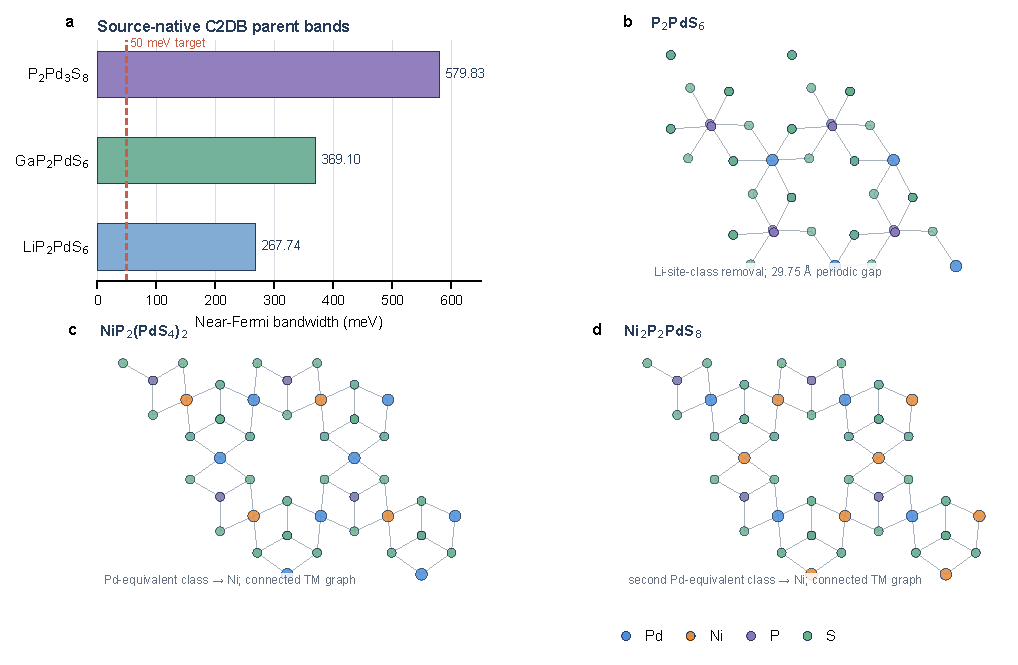
\includegraphics[width=\linewidth]{figures/prompt1-real-structures-v2.pdf}
    \caption{\textbf{Database evidence followed by explicit structure generation in the two-dimensional flat-band study.}
    (a) Source-native C2DB bands establish the bandwidth scale of the three parent structures.  (b--d) Top-view projections rendered from the generated CIF artifacts for the three children admitted by the structural hard gates.  The structures, values, and lineages are taken from the archived run; the plotting layout is generated separately for this report.}
    \label{fig:prompt1}
\end{figure}

\begin{table}[t]
    \centering
    \caption{\textbf{Structure-backed hypotheses generated in case study I.}}
    \label{tab:prompt1-children}
    \small
    \setlength{\tabcolsep}{4pt}
    \renewcommand{\arraystretch}{1.13}
    \begin{tabularx}{\linewidth}{>{\raggedright\arraybackslash}p{0.19\linewidth}>{\raggedright\arraybackslash}p{0.18\linewidth}XX}
        \toprule
        \textbf{Parent} & \textbf{Child} & \textbf{Compiled operation} & \textbf{Structure-level outcome} \\
        \midrule
        LiP$_2$PdS$_6$ & P$_2$PdS$_6$ & Remove complete Li site class & 2D, connected Pd graph, common Pd(II) \\
        P$_2$Pd$_3$S$_8$ & NiP$_2$(PdS$_4$)$_2$ & First Pd class $\rightarrow$ Ni & 2D, connected Ni/Pd graph, common Ni(II)/Pd(II) \\
        P$_2$Pd$_3$S$_8$ & Ni$_2$P$_2$PdS$_8$ & Second Pd class $\rightarrow$ Ni & 2D, connected Ni/Pd graph, common Ni(II)/Pd(II) \\
        GaP$_2$PdS$_6$ & GaNi(PS$_3$)$_2$ & Pd class $\rightarrow$ Ni & Structure retained as a charge-compensation revision route \\
        \bottomrule
    \end{tabularx}
\end{table}

This study exercises the full transition from retrieved electronic evidence to new structure records.  It also demonstrates the distinction between stages: passing the structure gates promotes a child into an electronic-screening portfolio, while the 50\,meV and orbital-character constraints remain attached as model targets.  The final products are therefore three explicit, reproducible structures and one revised chemical route, rather than a list of text-only substitutions.

\subsection{Case study II: van der Waals ferromagnetic topological materials}
\label{sec:case-vdw}

\paragraph{Goal.}
The second case asks for layered materials that combine ferromagnetism with a non-trivial spin--orbit-coupled insulating state.  \matspec decomposed the request into magnetic ground-state energy, ordering scale, SOC gap, Fermi-level placement, and a topological invariant.  Rather than reduce the search to a single chemical family, \matevidence and \mattransform organized six routes that act on different physical levers established by two-dimensional magnets and magnetic topological materials \cite{gong2017cgt,huang2017cri3,otrokov2019mnbi2te4,rienks2019hetero}.

\begin{figure}[H]
    \centering
    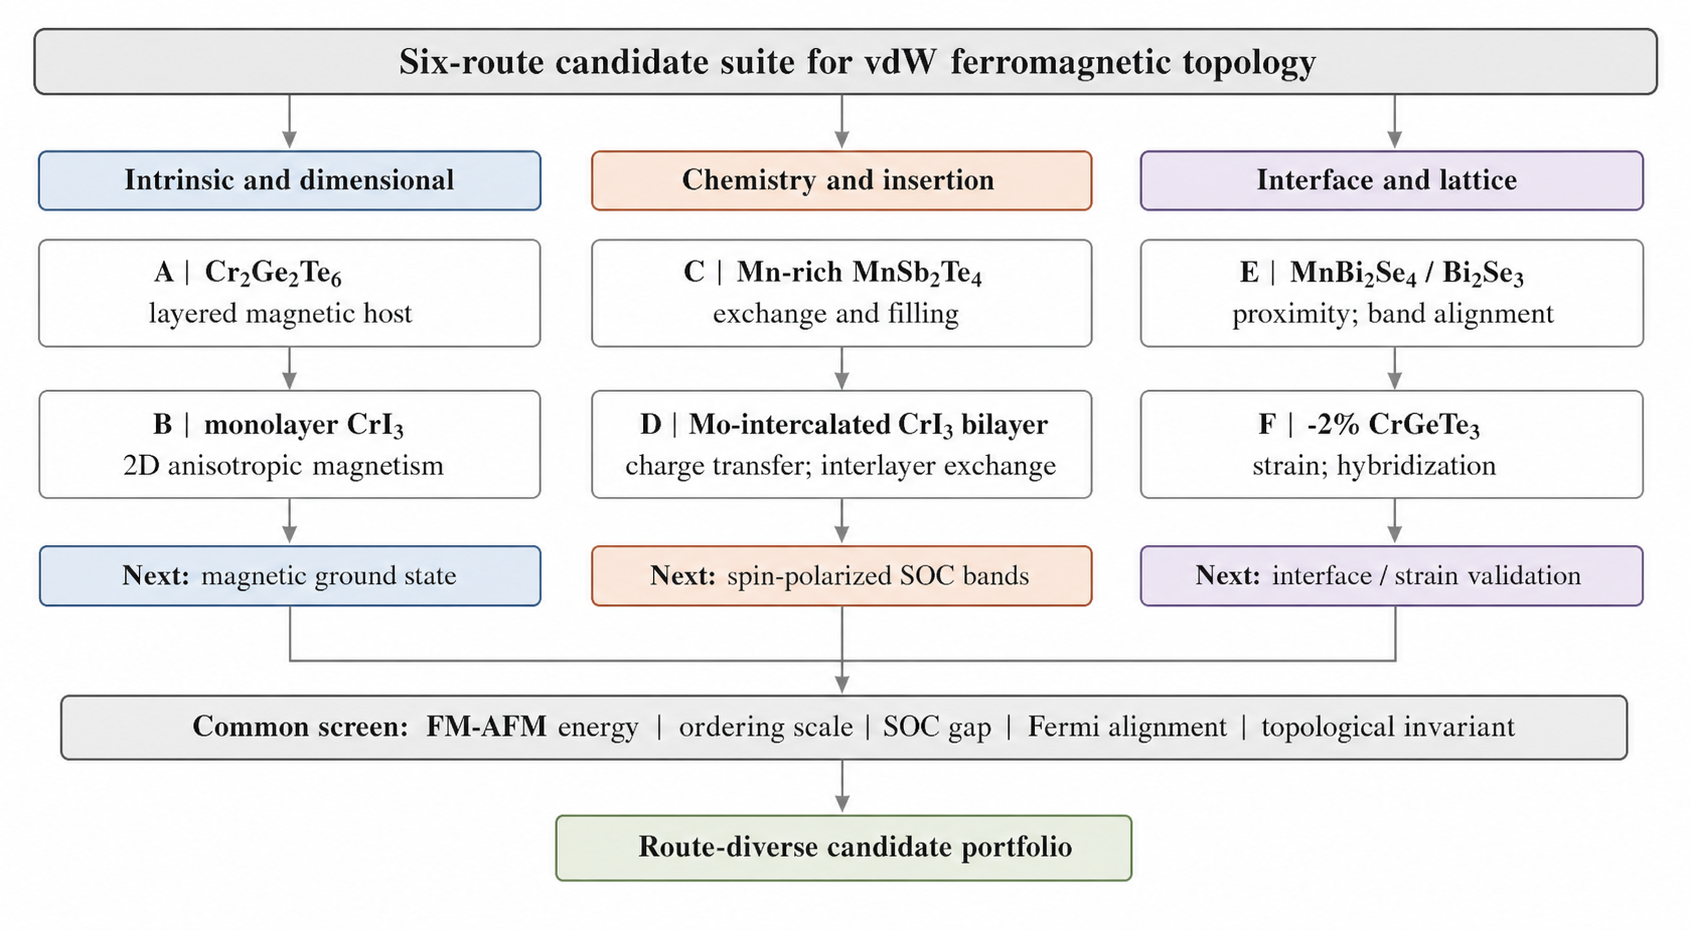
\includegraphics[width=0.88\linewidth]{figures/vdw-six-routes-image2-v3.png}
    \caption{\textbf{Six-route exploration of van der Waals ferromagnetic topology.}
    The portfolio spans intrinsic magnetic hosts, the monolayer limit, magnetic stoichiometry, intercalation, proximity coupling, and strain.  Every route is evaluated against the same five-observable verification matrix, allowing chemically distinct candidates to remain comparable.  The experiment-suite layout follows the compact evidence-column grammar used in AutoSci; the Image2-generated conceptual summary contains candidate identities and route definitions taken from the archived campaign.}
    \label{fig:vdw-routes}
\end{figure}

The intrinsic-host route retained Cr$_2$Ge$_2$Te$_6$ as a layered magnetic starting point.  The monolayer route used CrI$_3$ to focus on the dimensional dependence of ferromagnetism.  A Mn-rich MnSb$_2$Te$_4$ route varied magnetic stoichiometry in a tetradymite-related setting.  A Mo-intercalated CrI$_3$ bilayer instantiated charge-transfer and interlayer-exchange control as an intercalation plan.  A MnBi$_2$Se$_4$/Bi$_2$Se$_3$ route represented magnetic proximity and band-alignment control at a van der Waals interface.  Finally, a $-2\%$ CrGeTe$_3$ route encoded homogeneous strain as a direct structural operation.

\begin{table}[t]
    \centering
    \caption{\textbf{Route portfolio for case study II.}}
    \label{tab:vdw-routes}
    \small
    \setlength{\tabcolsep}{3.5pt}
    \renewcommand{\arraystretch}{1.12}
    \begin{tabularx}{\linewidth}{>{\raggedright\arraybackslash}p{0.20\linewidth}>{\raggedright\arraybackslash}p{0.22\linewidth}XX}
        \toprule
        \textbf{Route} & \textbf{Candidate realization} & \textbf{Primary physical lever} & \textbf{Decisive next calculation} \\
        \midrule
        Intrinsic host & Cr$_2$Ge$_2$Te$_6$ & Native layered magnetism and heavy-ligand SOC & Magnetic order plus SOC topology in the same state \\
        Monolayer limit & CrI$_3$ monolayer & Dimensionality and anisotropy & Magnetic ground state, gap and Fermi placement \\
        Stoichiometry & Mn-rich MnSb$_2$Te$_4$ & Exchange and filling through magnetic content & Competing magnetic configurations and invariant \\
        Intercalation & Mo--CrI$_3$ bilayer & Charge transfer and interlayer exchange & Relaxed registry followed by spin-polarized SOC bands \\
        Proximity & MnBi$_2$Se$_4$/Bi$_2$Se$_3$ & Exchange transfer across a vdW interface & Interface band alignment and topological invariant \\
        Strain & $-2\%$ CrGeTe$_3$ & Band inversion, hybridization and anisotropy & Strain-resolved FM--AFM energy and SOC gap \\
        \bottomrule
    \end{tabularx}
\end{table}

The route map is the principal result of this campaign stage.  Each candidate carries a different mechanism, but all share the same evidence schema and verification targets.  This makes it possible to allocate subsequent calculations by information gain: magnetic-energy calculations for routes with unresolved order, SOC calculations for candidates with an established magnetic state, and interface relaxation before electronic claims for proximity and heterostructure routes.  The system thus preserves scientific diversity without losing a common definition of success.

\subsection{Case study III: fractional-valence transition metals on a Lieb lattice}
\label{sec:case-lieb}

\paragraph{Goal.}
The third case poses an open problem: identify a crystalline material in which fractionally valent transition metals form a Lieb lattice and contribute a flat band at the Fermi level.  The compiled target requires (i) an explicit structure, (ii) non-integer average transition-metal valence compatible with charge balance, (iii) periodic Lieb connectivity of the contributing sites, (iv) a near-Fermi band width no greater than 50\,meV, (v) no disqualifying dispersive or first-order crossing, and (vi) transition-metal or hybridized ligand orbital weight.  The target connects crystalline flat-band classification, crystal-net catalogues, and electronic Lieb-lattice realizations \cite{calugaru2022flatbands,neves2024crystalnets,drost2017lieb}; no single source exposes the complete conjunction.

The campaign therefore ran three complementary routes.  The federated-database route returned 24 structures and developed seven candidate hypotheses, including cuprate, nickelate, and Pt--P/oxide-derived families.  The literature-and-mechanism route resolved 103 evidence records around six hypotheses, with layered oxyhalides such as NbOCl$_2$ and TaOCl$_2$, Ba$_2$CuO$_{3+\delta}$-related systems, and metal--inorganic-framework Lieb nets as mechanism anchors.  The structure-generation route began from three explicit database parents and produced eight intervention hypotheses, including alkali intercalation, halogen vacancy control, electrostatic gating, tensile strain, and framework routes.

The three routes were merged by candidate identity and structural lineage before model routing.  Across the consolidated campaign, 21 hypotheses yielded 17 unique structures with complete learned-Hamiltonian and band executions.  Seven operator executions produced six unique registry-child CIFs.  Four literature hypotheses without resolved structures remained linked to their mechanisms and structure-acquisition targets rather than being sent to a model with no input.

\begin{table}[t]
    \centering
    \caption{\textbf{Three-route coverage in the Lieb-lattice study.}}
    \label{tab:lieb-routes}
    \small
    \setlength{\tabcolsep}{4pt}
    \renewcommand{\arraystretch}{1.13}
    \begin{tabularx}{\linewidth}{>{\raggedright\arraybackslash}p{0.19\linewidth}c c X}
        \toprule
        \textbf{Route} & \textbf{Database leads} & \textbf{Hypotheses} & \textbf{Distinct contribution} \\
        \midrule
        Federated database & 24 & 7 & Broad structure-backed candidate discovery across four databases \\
        Literature route & 24 & 6 & Oxyhalide, cuprate and framework mechanisms linked to persistent papers and structures \\
        Structure generation & 3 & 8 & Intercalation, vacancy, gate, strain and framework interventions \\
        \midrule
        Consolidated ML campaign & \multicolumn{2}{c}{17 unique structures executed} & SOC learned-Hamiltonian bands and common hard diagnostics \\
        \bottomrule
    \end{tabularx}
\end{table}

The learned-Hamiltonian screen measured the narrowest near-Fermi band for each structure under a common 50\,meV policy.  The current closest structures were three Li$_2$Ni$_5$OF$_{11}$ vacancy-derived children with bandwidths of 60.134, 63.576, and 147.073\,meV, an NbCl$_2$O structure at 64.648\,meV, and TaCl$_2$O at 88.852\,meV.  These values re-prioritize the candidate set toward the Li--Ni oxyfluoride and oxyhalide branches.  The same band diagnostics also identify competing crossings, which become the target of the next structure and filling modifications.

\begin{figure}[H]
    \centering
    \begin{subfigure}[t]{0.48\linewidth}
        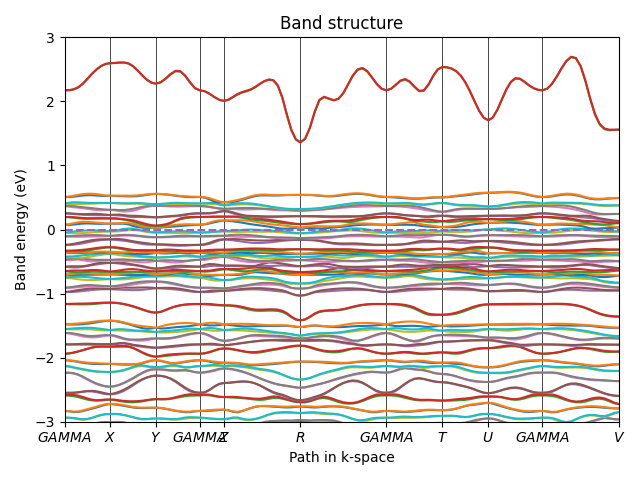
\includegraphics[width=\linewidth]{figures/lieb-li2ni5of11-band.png}
        \caption{Li$_2$Ni$_5$OF$_{11}$ child, $W=60.134$\,meV.}
    \end{subfigure}\hfill
    \begin{subfigure}[t]{0.48\linewidth}
        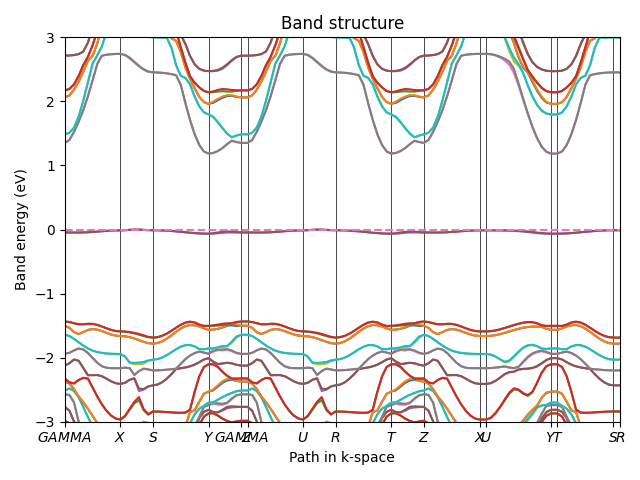
\includegraphics[width=\linewidth]{figures/lieb-nbcl2o-band.png}
        \caption{NbCl$_2$O, $W=64.648$\,meV.}
    \end{subfigure}

    \begin{subfigure}[t]{0.48\linewidth}
        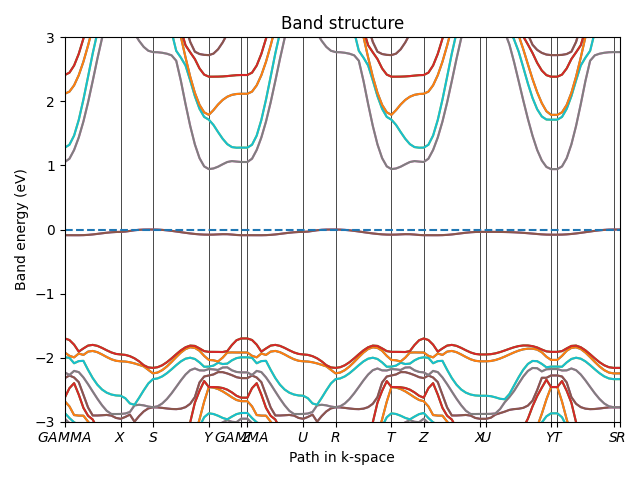
\includegraphics[width=\linewidth]{figures/lieb-tacl2o-band.png}
        \caption{TaCl$_2$O, $W=88.852$\,meV.}
    \end{subfigure}\hfill
    \begin{subfigure}[t]{0.48\linewidth}
        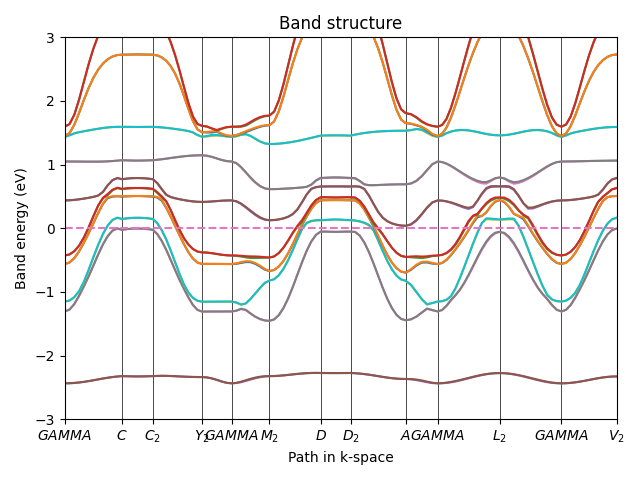
\includegraphics[width=\linewidth]{figures/lieb-nbcl2f-band.png}
        \caption{NbCl$_2$F substitution child, $W=1.454$\,eV.}
    \end{subfigure}
    \caption{\textbf{Candidate-specific SOC learned-Hamiltonian band artifacts from the Lieb-lattice campaign.}
    The panels are native archived outputs, not illustrative reconstructions.  The screen resolves bandwidth and band-crossing diagnostics for each exact structure.  Orbital projection, contributor-site Lieb connectivity, charge distribution, and model calibration remain separate validation targets.}
    \label{fig:lieb-bands}
\end{figure}

Figure~\ref{fig:lieb-bands} shows representative native band artifacts.  The NbOCl$_2$$\rightarrow$NbCl$_2$F example illustrates why explicit structure realization matters: replacing the complete O-equivalent class creates the $x=1$ end member, and the computed band is correspondingly attached to NbCl$_2$F rather than to an unspecified mixed NbO$_{1-x}$F$_x$Cl$_2$.  Intermediate filling now has a concrete next operation---ordered partial substitution in a supercell or a condition-level doping plan---and a parent observation against which descendants can be compared.

The campaign converts a broad open question into a compact experimental and computational frontier.  Li$_2$Ni$_5$OF$_{11}$ descendants are prioritized for charge analysis, orbital projection, and modifications intended to remove the competing Fermi crossing.  NbCl$_2$O and TaCl$_2$O are prioritized for contributor-sublattice connectivity and calibrated electronic confirmation.  Framework hypotheses retain structure acquisition as their next gate.  In every case, the next step is attached to a structure and to the constraint it is intended to resolve.

\subsection{Cross-case system evaluation}
\label{sec:evaluation}

The three studies test whether the same architecture can preserve scientific objects across qualitatively different workflows.  Table~\ref{tab:crosscase} summarizes the observed artifact coverage.  Case I emphasizes source bands, structural transformation, and parent--child provenance.  Case II emphasizes route diversity and a shared verification matrix.  Case III combines all three discovery routes with explicit model execution and iterative structure lineage.

\begin{table}[t]
    \centering
    \caption{\textbf{Cross-case artifact coverage.}}
    \label{tab:crosscase}
    \small
    \setlength{\tabcolsep}{3.5pt}
    \renewcommand{\arraystretch}{1.13}
    \begin{tabularx}{\linewidth}{>{\raggedright\arraybackslash}p{0.20\linewidth}>{\raggedright\arraybackslash}p{0.20\linewidth}XX}
        \toprule
        \textbf{Case} & \textbf{Route and plan coverage} & \textbf{Scientific artifacts} & \textbf{Portfolio output} \\
        \midrule
        2D TM flat band & 1 route; 4 compiled child plans & 3 source bands and 4 child CIFs & Three structure-screening children and one revision route \\
        vdW FM topology & 6 route-bound structure or interface plans & Six candidate verification matrices & Route-diverse portfolio with five shared observables \\
        Fractional-valence Lieb lattice & 3 routes; 7 operator executions; 6 unique children & 17 learned-Hamiltonian band runs & Ranked structure frontier and observable-specific next tasks \\
        \bottomrule
    \end{tabularx}
\end{table}

We use five object-level criteria.  \emph{Constraint coverage} is the fraction of compiled constraints represented in the candidate matrix, including UNKNOWN entries.  \emph{Provenance completeness} requires each populated observation to resolve to a source or execution artifact.  \emph{Structure-backed hypothesis rate} measures which chemical modifications bind to a parent and an executable plan or condition realization.  \emph{Model-route executability} measures whether an approved task has all required input and capability bindings.  \emph{Research continuity} measures whether outputs from one cycle can be consumed without re-entering candidate identity, structure, or evidence manually.  The archived campaigns achieve complete schema coverage and artifact linkage by construction; the case-specific counts in Table~\ref{tab:crosscase} describe how much scientific work was instantiated beyond that contract.

\subsection{Layered comparison and expert benchmark protocol}
\label{sec:benchmark}

To separate the contributions of the language model, \hermes, and the materials service, we define a paired layered benchmark with five arms: base model only; base model with the \hermes research harness; \hermes with retrieval and federated evidence; \hermes plus evidence and \mattransform; and the complete system with \matdag and \matevolve.  Cases are grouped by structure family before assignment so that near-duplicate derivatives do not enter opposite arms.  Each arm receives the same scientific prompt, time budget, accessible public evidence, and output template.

The primary evaluation unit is the candidate-level deliverable, scored on scientific constraint fidelity, source correctness, candidate identity, structural executability, validation specificity, and expert usefulness.  Runtime, tool calls, recovered artifacts, and coverage of decisive observables are recorded as secondary measures.  Expert scoring is performed independently on blinded reports, followed by adjudication of disagreements and a bootstrap confidence interval over source-family groups.

The pre-case calibration contained 12 candidate cases.  After structure-family deduplication and target-class eligibility screening, five independent cases remained for rubric calibration, producing 36 item-level disagreements for adjudication.  This calibration established the scoring manual and blinding workflow.  The report does not convert those calibration judgements into a comparative performance claim; the paired scientific benchmark is reported only when the frozen eligible pool and compute budget support the planned analysis.  The current manuscript therefore grounds its system claims in the end-to-end artifacts above and treats the layered benchmark as the registered evaluation protocol for the next release.

\subsection{Component analysis}

The case studies make the expected contribution of each module observable.  Removing \matspec collapses compound goals into loosely phrased search terms and eliminates a common denominator across routes.  Removing \matevidence loses candidate-linked provenance and conflates direct observations with inference.  Removing \mattransform preserves suggestions but removes child CIFs and parent--child comparison.  Removing \matdag produces structures without capability-checked observables.  Removing \matevolve prevents subsequent cycles from acting on the structures and unresolved constraints already produced.  Removing \hermes leaves the domain service callable, but loses the natural-language research interaction, Profile/Skill policy, controlled continuation, and workflow-level evolution that make the platform usable as a persistent agent.

These are structural ablations of the artifact graph, not substitutions of one model score for another.  They define the rows of the paired benchmark and explain why the complete platform is evaluated on scientific deliverables rather than response fluency alone.

\section{Related Work}
\label{sec:related}

\subsection{Agentic systems for scientific research}

Tool-augmented language models have moved scientific agents from conversational assistance toward the execution of specialist workflows.  ChemCrow connects a language model to chemistry tools and demonstrates improvements on synthesis, safety, and analysis tasks \cite{bran2024chemcrow}.  Coscientist organizes language models, web search, code execution, and laboratory hardware to plan and execute chemical experiments \cite{boiko2023coscientist}.  A-Lab combines literature-derived synthesis knowledge, active learning, computation, and robotics in an autonomous inorganic-synthesis loop \cite{szymanski2023alab}.  More recent co-scientist systems use interacting agents and scientist feedback to generate and refine hypotheses \cite{gottweis2026coscientist}.

These systems motivate research agents as coordinators rather than standalone predictors.  AutoSci extends this view to a complete research lifecycle organized around long-term knowledge memory, active research memory, a staged harness, reusable DAG operators, and controlled self-evolution \cite{qian2026autosci}.  \system adopts the lifecycle perspective while changing the persistent unit from a general research entity to a structure-centred materials candidate.  Its candidate record makes crystal structures, transformation lineages, model inputs, and observable-level evidence directly addressable throughout the lifecycle.

\subsection{Materials data federation}

Large computational databases provide the substrate for modern materials screening.  The Materials Project supplies computed structures and properties through a programmatic interface \cite{jain2013materials}; C2DB specializes in systematically calculated two-dimensional materials and electronic structures \cite{haastrup2018c2db}; NOMAD provides FAIR storage and analysis of heterogeneous computational materials data \cite{sbailo2022nomad}; and MC3D curates experimentally known inorganic structures and reproducible DFT relaxations \cite{huber2026mc3d}.  OPTIMADE defines a common API that enables interoperable access across database providers \cite{andersen2021optimade}.

Federation creates a semantic problem in addition to an access problem.  The same formula may refer to several polymorphs, magnetic configurations, dimensional reductions, or calculation levels, while a property available in one source may not exist in another.  \matevidence therefore retains source identities and native provenance, links records through explicit candidate-identity edges, and does not fill missing candidate properties by cross-database analogy.  The resulting evidence graph complements standards for data exchange by defining how retrieved records become candidate-specific scientific judgements.

\subsection{Materials generation and structure intervention}

Machine-learning models have substantially expanded candidate generation.  GNoME uses deep learning and large-scale first-principles evaluation to identify stable crystal structures \cite{merchant2023gnome}; MatterGen generates inorganic materials under compositional, symmetry, and property conditions \cite{zeni2025mattergen}; and SCIGEN integrates structural constraints into generative modelling for quantum-material motifs such as Lieb lattices \cite{okabe2026scigen}.  These models address the important inverse problem of proposing crystals from learned structure distributions.

\mattransform addresses a complementary task.  It begins from an identified parent and compiles a scientific intervention---substitution, removal, intercalation, strain, layer sliding, doping, gating, proximity, or heterostructure formation---into a typed operation or condition plan.  Its primary object is the parent--operation--child lineage rather than an isolated generated sample.  This formulation is particularly useful for soft-chemistry reasoning, in which the relationship to a known parent, charge-compensation route, stacking arrangement, or experimental control variable is part of the hypothesis.

\subsection{Accelerated atomistic and electronic models}

Machine-learning interatomic potentials offer rapid access to energies, forces, and structural relaxation.  CHGNet incorporates magnetic moments as a charge-informed representation and is pretrained on Materials Project trajectories \cite{deng2023chgnet}.  Learned electronic models target a different layer of the scientific stack.  Uni-HamGNN predicts spin--orbit-coupled Hamiltonians across broad chemistry and supplies an accelerated route to quantum-material bands \cite{zhong2026uniham}.  First-principles packages such as Quantum ESPRESSO remain central for higher-specificity electronic calculations and controlled validation \cite{giannozzi2017qe}.

\matdag treats these programs as capabilities with different inputs, observables, domains, and evidence ceilings.  A structure model, Hamiltonian model, band analyser, and first-principles calculation can therefore appear in one dependency graph without making their outputs interchangeable.  The graph is assembled for each candidate and each unresolved constraint, allowing accelerated screening to narrow a portfolio before selected higher-cost calculations.

\subsection{Flat bands, Lieb lattices, and magnetic topology}

Crystalline flat bands provide a structural route to enhanced interactions and non-trivial topology.  General classifications connect flat bands to real-space band representations and lattice geometry \cite{calugaru2022flatbands}, while high-throughput crystal-net catalogues identify large numbers of elemental sublattices with model flat bands, including Lieb nets \cite{neves2024crystalnets}.  Electronic Lieb lattices have also been constructed and imaged in atomically patterned surface systems \cite{drost2017lieb}.  These works motivate combining graph-level lattice recognition with explicit electronic and orbital diagnostics.

Layered magnetic materials provide a complementary design space.  Intrinsic ferromagnetism in few-layer Cr$_2$Ge$_2$Te$_6$ and layer-dependent ferromagnetism in CrI$_3$ established two-dimensional van der Waals magnets as experimentally accessible systems \cite{gong2017cgt,huang2017cri3}.  MnBi$_2$Te$_4$ and related heterostructures demonstrate how magnetic order, spin--orbit coupling, surfaces, and interfaces can jointly produce topological electronic states \cite{otrokov2019mnbi2te4,rienks2019hetero}.  The six-route case study in Section~\ref{sec:case-vdw} uses these physical mechanisms as search axes while retaining separate magnetic, band-alignment, and topological observables.

\subsection{Positioning}

\system lies at the intersection of these areas.  It is not a new foundation model, a single materials database, or a replacement for a first-principles code.  It is a persistent research environment that turns an open scientific question into a candidate-centred graph of constraints, evidence, structures, operations, model tasks, and decisions.  Its contribution is the shared abstraction that lets agentic research, materials federation, soft-chemistry structure realization, and heterogeneous scientific models operate on the same evolving materials objects.

\section{Conclusion and Outlook}
\label{sec:conclusion}

We presented \system, a persistent materials-research platform built on the \hermes agent runtime.  The system couples a controlled natural-language research environment to a structure-centred scientific service through a bounded MCP interface.  Five domain modules give the platform its scientific semantics: \matspec compiles open questions into constraint graphs; \matevidence aligns literature and federated database evidence around stable candidate identities; \mattransform realizes soft-chemistry proposals as typed structure operations or condition plans; \matdag constructs capability-aware scientific task graphs; and \matevolve carries candidate lineages and validation state into subsequent cycles.

The three case studies demonstrate the breadth of this formulation.  In the two-dimensional flat-band study, source-native database bands led directly to four explicit child structures and a structure-screened portfolio.  In the van der Waals ferromagnetic-topology study, the system organized six physically distinct routes under one five-observable verification matrix.  In the fractional-valence Lieb-lattice study, federated database discovery, literature-and-mechanism transfer, and structure generation converged into 21 hypotheses, 17 executed structures, six unique registry children, and a candidate-specific learned-Hamiltonian frontier.  The nearest current candidates---Li$_2$Ni$_5$OF$_{11}$ descendants and NbCl$_2$O/TaCl$_2$O oxyhalides---now have explicit next tasks for orbital character, charge distribution, lattice connectivity, crossing removal, and calibrated electronic confirmation.

These results show why a materials agent benefits from persistent scientific objects.  Evidence can remain incomplete without losing provenance; a proposed chemical change can become a reproducible child structure; a model result can update only the constraint it actually measures; and the next cycle can operate on the same candidate rather than reconstructing it from dialogue.  \hermes supplies interaction, policy, continuation, and workflow evolution, while the materials layer supplies the candidate, structure, evidence, and task semantics needed for scientific continuity.

The next release will extend this foundation in three directions.  First, structure generation will add ordered-supercell and partial-occupancy enumeration so that fractional substitution and mixed valence can be realized between end members.  Second, the electronic route will add orbital-resolved projections, contributor-sublattice graph validation, topological invariants, and calibrated uncertainty for learned Hamiltonians, followed by selected first-principles confirmation.  Third, the frozen layered benchmark will be executed on an expanded structure-family-independent case pool, enabling paired expert evaluation of the base model, \hermes harness, evidence layer, structure layer, and complete system.  These additions preserve the same candidate-centred contract and extend the set of scientific questions that can be resolved within it.

By placing evidence, structure manipulation, computation, and research evolution in one durable graph, \system provides a practical route from an open materials question to an explicit and progressively testable materials hypothesis.

\appendix

\section{Hermes Profiles and Gateway Surface}
\label{app:hermes}

The repository contains three source-controlled \hermes Profiles.  \texttt{materials-inspiration} exposes the production materials and research toolsets with manual approvals and bounded run continuation.  \texttt{materials-inspiration-research} exposes the long-running generic research entry point.  \texttt{materials-inspiration-evolution} enables \hermes-native Skills, memory, curator, and bounded delegation while exposing only read-only materials run and result tools.  The deployment used \hermes release v2026.8.3, package version 0.20.0.

The production MCP surface contains four core actions: start an inspiration run, read run state, apply an advertised run action, and retrieve a verified terminal result.  Research Profiles additionally expose the complete materials-research pipeline and generic research entry points.  Each tool validates strict JSON input and output models.  Read-only tools are distinguished from mutating tools, and result retrieval verifies the authoritative terminal artifact before returning its projection.  The exact public tool identifiers are retained in the source-controlled Profile manifests.

\section{Candidate and Evidence Contracts}
\label{app:contracts}

A candidate record contains a stable candidate identifier, source identities, formula, structure pointers, route, constraint matrix, inference matrix, operation plans, model tasks, and decision history.  An evidence record minimally contains the candidate identifier, constraint identifier, relation, value and units where applicable, source or model identity, artifact pointer, retrieval or execution time, and provenance hash.  Direct evidence verdicts are PASS, FAIL, or UNKNOWN.  Scientific inference is stored separately as LIKELY\_PASS or LIKELY\_FAIL with confidence, assumptions, and a decisive falsifier.

Structures are content-addressed.  Cross-database identity links do not merge native entries or their properties; they add typed edges between source records and the candidate.  A model observation is attached to the exact structure artifact used as input.  This contract prevents a family-level paper, parent property, or neighbouring database entry from becoming a child-specific numerical observation.

\section{Soft-Chemistry Registry}
\label{app:softchem}

The registry resolves the following versioned operators:

\begin{itemize}
    \item \texttt{SUBSTITUTE\_EQUIVALENT\_SITE\_V1};
    \item \texttt{REMOVE\_EQUIVALENT\_SITE\_CLASS\_V1};
    \item \texttt{INTERCALATE\_REASONED\_GAP\_SITE\_V1};
    \item \texttt{APPLY\_HOMOGENEOUS\_STRAIN\_V1};
    \item \texttt{SLIDE\_REASONED\_LAYER\_V1};
    \item \texttt{APPLY\_CARRIER\_DOPING\_V1};
    \item \texttt{APPLY\_ELECTROSTATIC\_GATE\_V1};
    \item \texttt{PLAN\_MAGNETIC\_PROXIMITY\_V1};
    \item \texttt{PLAN\_VDW\_HETEROSTRUCTURE\_V1}.
\end{itemize}

Every plan freezes its operator and specification version, typed parameters, parent structure pointer, scientific rationale, provenance, and canonical content hash.  Structure outputs pass parse, CIF round-trip, coordinate, cell, site-count, minimum-distance, dimensionality, periodic-gap, and contributor-graph checks as applicable.  Chemistry priors report charge-balance and common-valence assessments without replacing electronic calculations.

\section{Scientific Task and Artifact Types}
\label{app:tasks}

The validation service defines task kinds for research-evidence import, database band import, two-dimensional structure assessment, generic model inference, structure/energy models, learned non-SOC and SOC Hamiltonians, band calculation, band analysis, and first-principles execution.  Input and output artifacts include canonical CIFs, source responses, graph inputs, checkpoints, Hamiltonian arrays, band arrays and plots, normalized observations, execution receipts, and scientific evidence records.

Capabilities declare supported task kinds and observables, accepted and required artifacts, produced artifacts, physics features, supported chemistry or dimensionality when constrained, checkpoint hash, benchmark status, evidence ceiling, real-backend status, and cost.  A route is approved only when its input structure, prerequisite artifacts, parameter schema, capability snapshot, and cost satisfy the frozen policy.

\section{Backend Controls}
\label{app:controls}

Three end-to-end controls exercise independent portions of the scientific stack.  A CHGNet calculation ran on an NVIDIA L40S and returned a real energy/force result for elemental Si, establishing device selection, checkpoint loading, artifact transfer, and receipt capture for the structure-model adapter.  A Uni-HamGNN route produced a real SOC Hamiltonian and band structure for ZrSiPt; the archived band analysis measured a target bandwidth of 0.827865\,eV.  A remote Quantum ESPRESSO 7.6 self-consistent-field run for Si produced a total energy of $-16.51510414$\,Ry and preserved its calculation manifest and remote outputs.  These controls validate adapter execution and provenance within their stated systems and observables.

\section{Layered Benchmark Protocol}
\label{app:benchmark}

The paired benchmark evaluates five arms: base language model; base model with \hermes; \hermes with retrieval and federated evidence; \hermes with evidence and structure transformations; and the complete system with model DAG and candidate evolution.  Assignment operates at the structure-family group level.  The frozen rubric scores scientific constraint fidelity, source correctness, candidate identity, structural executability, validation specificity, and expert usefulness.  Runtime, model/tool calls, artifact recovery, and decisive-observable coverage are secondary measures.

Reports are blinded before independent expert review.  Adjudication records item-level disagreements without changing the original reviews.  Analysis uses paired case-level differences and bootstrap intervals over structure-family groups.  Calibration used 12 pre-cases; five independent eligible cases were retained after structure-family and target-class screening, and 36 item-level disagreements were adjudicated to finalize the rubric.

\section{Reproducibility and Artifact Layout}
\label{app:reproducibility}

Each run directory contains the original request, normalized goal and constraint graph, source query receipts and raw responses, candidate and evidence records, structure artifacts, operator plans and results, capability snapshots, model task plans, execution bindings, native outputs, normalized scientific evidence, feedback cycles, and a terminal report.  Content hashes bind plans and observations to exact inputs.  Run identifiers and idempotent task identities permit recovery without overwriting prior artifacts.

The conceptual system figures in this manuscript are generated separately from the scientific results, and their prompts are retained with the figure files.  Statistical plots are generated from manuscript source-data tables and exported as editable SVG/PDF plus high-resolution raster formats.  Structure panels are rendered from archived CIFs, and band panels reproduce archived model outputs directly.


\bibliographystyle{unsrtnat}
\bibliography{references}

\end{document}
